% ---------------------------------------------------------------------------------------------------------------
%                       TEMPLATE PARA TRABALHO DE CONCLUSÃO DE CURSO
% ---------------------------------------------------------------------------------------------------------------
% Projeto Original: Template com Customização da classe abnTeX2 para as normas da UTFPR 
% Autores: Diego Marczal
% 	       Michael Vornes <https://github.com/mvornes>
%
% Modificado por: Gabriel Cabral
%----------------------------------------------------------------------------------------------------------------
% Codificação: UTF-8
% LaTeX:  abnTeX2
% ---------------------------------------------------------------------------------------------------------------

% ---------------------------------------------------------------------------------------------------------------
%                                          CARREGA CLASSE PERSONALIZADA
% ---------------------------------------------------------------------------------------------------------------
\documentclass[%twoside,                   % Impressão em frente e verso
    	        oneside,                   % Impressão apenas frente
]{configuracoes/norma-abntex2}

% ---------------------------------------------------------------------------------------------------------------
%                                        INCLUI ARQUIVOS DE CONFIGURAÇÕES
% ---------------------------------------------------------------------------------------------------------------
\input{configuracoes/pacotes}
\input{configuracoes/config-pdf}

% ---------------------------------------------------------------------------------------------------------------
%                                 INCLUI ARQUIVOS DO TRABALHO DE CONCLUSÃO DE CURSO
% ---------------------------------------------------------------------------------------------------------------

% Insere capa e folha de rosto
% ----------------------------------------------------------------------------
%                                   CAPA
% ----------------------------------------------------------------------------
% Caso algum dos campos não se aplique ao seu trabalho, como por exemplo,
% se não houve coorientador, apenas deixe vazio.
% Exemplos:
% \coorientador{}
% \departamento{}

% ----------------------------------------------------------------------------
%                               DADOS DO TRABALHO
% ----------------------------------------------------------------------------
\titulo{Desenvolvimento de um Sistema Web para Apoio ao Manejo Comportamental de Crianças com TDAH e TOD}
\autor{Suellen Maciel Dutra}
\autorcitacao{SOBRENOME, Nome} % Sobrenome em maiúsculo
\local{Brasília-DF}
\data{2026}
\projeto{Trabalho de Conclusão de Curso}
\tituloAcademico{Tecnologia em Sistemas para Internet}

% ----------------------------------------------------------------------------
%                               DADOS DA INSTITUIÇÃO
% ----------------------------------------------------------------------------
\instituicao{Instituto Federal de Brasília}
\departamento{\textit{Campus} Brasília}
\programa{Tecnologia em Sistemas para Internet}
\logoinstituicao{0.15}{dados/figuras/ifb-logo.png}

% ----------------------------------------------------------------------------
%                              DADOS DOS ORIENTADORES
% ----------------------------------------------------------------------------
\orientador[Orientador:]{Gustavo Henrique Dornelas de Deus} 
%\instOrientador{Instituição do orientador}

\input{estrutura/pre-textuais/folha-rosto}
\input{estrutura/pre-textuais/folha-aprovacao}

\setcounter{tocdepth}{3}
\begin{document}

    \pretextual
    \imprimircapa                                     % Comando para imprimir Capa
    \imprimirfolhaderosto{}                           % Comando para imprimir Folha de rosto
    %\includepdf{ficha-catalografica.pdf}             % Comando para inserir Ficha catalográfica
    \imprimirfolhadeaprovacao{}                       % Comando para imprimir Folha de aprovação temporária
    
    % Insere elementos pré-textuais
    % ----------------------------------------------------------------------------
%                               DEDICATÓRIA
% ----------------------------------------------------------------------------

\renewcommand{\dedicatorianame}{DEDICATÓRIA}

\begin{dedicatoria}

    Dedico este trabalho a todas as pessoas neurodivergentes e às suas famílias, que lutam diariamente por inclusão, respeito e por um espaço no mundo. Que a tecnologia seja sempre uma ponte para a empatia, e nunca uma barreira. 

\end{dedicatoria}
          		% Dedicatória
    % ----------------------------------------------------------------------------
%                               AGRADECIMENTOS
% ----------------------------------------------------------------------------

\begin{agradecimentos}[AGRADECIMENTOS]

    Agradeço primeiramente a Deus, autor da vida, por ter me concedido saúde e perseverança para concluir esta jornada, sendo meu sustento nos momentos de maior desafio.

    À minha família, pelo apoio constante e por sempre torcerem pelo meu sucesso em cada etapa. O incentivo de vocês foi fundamental para que eu pudesse manter o foco nos estudos e alcançar esta conquista.
    
    Ao meu orientador, \orientador, a quem dedico um carinho e uma gratidão imensos. Obrigado por ter abraçado este projeto junto comigo desde o primeiro momento, por acreditar na relevância deste tema e por me guiar com tanta sabedoria, paciência e parceria. Sua orientação foi peça-chave para que esta ideia se transformasse em realidade.
    
    Ao meu cunhado, Pedro Dias Santana, e à minha aluna, Laura Lourenço, que convivem com o TDAH e o TOD. Vocês são a razão de ser deste trabalho. Agradeço por me ensinarem diariamente sobre resiliência e por me inspirarem a buscar soluções que tornem a educação um lugar mais acolhedor para todos. Suas histórias deram propósito e alma a cada linha escrita neste projeto.
    
    A todos os professores e colegas que fizeram parte desta trajetória e que, de alguma forma, contribuíram para o meu crescimento pessoal e profissional. Meu sincero agradecimento.

\end{agradecimentos}
        		% Agradecimentos
    % ----------------------------------------------------------------------------
%                                   EPÍGRAFE
% ----------------------------------------------------------------------------

\renewcommand{\epigraphname}{EPÍGRAFE}

\begin{epigrafe}

    \textit{``A inclusão acontece quando se aprende com as diferenças e não com as igualdades.''}\\
    \textbf{— Paulo Freire}

\end{epigrafe}

              		% Epígrafe
    % ----------------------------------------------------------------------------
%                                   RESUMO
% ----------------------------------------------------------------------------

\begin{resumo}[RESUMO]

    \begin{SingleSpacing}
    
        Este trabalho apresenta o desenvolvimento de um sistema web voltado ao auxílio no manejo comportamental de crianças diagnosticadas com Transtorno de Déficit de Atenção com Hiperatividade (TDAH) e Transtorno Opositor Desafiador (TOD). O objetivo central é promover a comunicação integrada entre pais e professores, de modo a alinhar estratégias de acompanhamento e reduzir inconsistências no processo educativo. A pesquisa parte da constatação de que a falta de comunicação eficaz entre família e escola compromete o desempenho acadêmico e social dessas crianças, além de gerar conflitos e dificultar a aplicação de intervenções consistentes. Quanto à metodologia científica, o estudo classifica-se como uma pesquisa tecnológica e aplicada. Para estruturar a solução, adota-se a prototipação como método de desenvolvimento, precedida pelo uso de instrumentos de pesquisa qualitativos — como a aplicação de questionários, entrevistas semiestruturadas e observação participante com a comunidade escolar — essenciais para o levantamento preciso de requisitos. A partir disso, o projeto busca oferecer funcionalidades para o registro ágil de comportamentos e o acompanhamento de estratégias pedagógicas proativas. A avaliação da ferramenta será conduzida posteriormente por meio de testes de usabilidade com usuários finais, garantindo a eficiência da interface. Os resultados esperados incluem a melhoria da comunicação entre os atores envolvidos, a redução da sobrecarga docente e o fortalecimento dos vínculos sociais, reforçando a importância da tecnologia voltada à inclusão e ao apoio no desenvolvimento infantil.
        
        \item\textbf{Palavras-chave}: Sistema web. Manejo comportamental. TDAH. TOD. Prototipação.
    
    \end{SingleSpacing}
    
\end{resumo}
             		% Resumo em Português
    % ----------------------------------------------------------------------------
%                                  ABSTRACT
% ----------------------------------------------------------------------------

\begin{resumo}[ABSTRACT]

    \begin{SingleSpacing}
    
       This work presents the development of a web-based system aimed at aiding behavioral management of children diagnosed with Attention Deficit Hyperactivity Disorder (ADHD) and Defiant Opposition Disorder (DOT). The central objective is to promote integrated communication between parents and teachers, in order to align strategies of accompaniment and reduce inconsistencies in the educational process. The research starts from the observation that the lack of effective communication between family and school compromises the academic and social performance of these children, in addition to generating conflicts and making it difficult to apply consistent interventions. As for the scientific methodology, the study is classified as a technological and applied research. To structure the solution, prototyping is adopted as a development method, preceded by the use of qualitative research instruments - such as the application of questionnaires, semi-structured interviews and participant observation with the school community - essential for accurate survey of requirements. From this, the project seeks to offer functionalities for the agile registration of behaviors and the monitoring of proactive pedagogical strategies. The evaluation of the tool will be conducted later through usability tests with end users, ensuring the efficiency of the interface. The expected results include improved communication between stakeholders, reduction of teacher overload and strengthening of social bonds, reinforcing the importance of technology aimed at inclusion and support in child development.
        
        \item\textbf{Keywords}: Web system. Behavioral management. ADHD. TOD. Prototyping.
    
    \end{SingleSpacing}
    
\end{resumo}
             		% Resumo em Inglês
    \include{estrutura/pre-textuais/listas/lista-figuras}       % Lista de Figuras
    \include{estrutura/pre-textuais/listas/lista-quadros}       % Lista de Quadros
    \include{estrutura/pre-textuais/listas/lista-tabelas}       % Lista de Tabelas
    % ----------------------------------------------------------------------------
%                       LISTA DE ABREVIATURAS E SIGLAS
% ----------------------------------------------------------------------------
% Altere a lista para definir os acrônimos e siglas utilizados neste trabalho

\begin{siglas}
    \item[ABNT] Associação Brasileira de Normas Técnicas
    \item[BaaS] Banco como Serviço
    \item[CSS3] Cascading Style Sheets
    \item[ECA] Estatuto da Criança e do Adolescente
    \item[HTML5] Hypertext Markup Language, versão 5
    \item[IDE] Ambiente de Desenvolvimento Integrado
    \item[IF] Instituto Federal de Educação, Ciência e Tecnologia
    \item[IFB] Instituto Federal de Educação, Ciência e Tecnologia de Brasília
    \item[LGPD]Lei Geral de Proteção de Dados Pessoais
    \item[UI] Interface do Usuário
    \item[RF] Requisitos Funcionais
    \item[RFN] Requisitos Não Funcionais
    \item[RU] Requisitos de Usuário
    \item[TCC] Trabalho de Conclusão de Curso
    \item[TDAH] Transtorno de Déficit de Atenção com Hiperatividade
    \item[TOD] Transtorno Opositor Desafiador
    \item[UC] Casos de Uso
    \item[UX] Experiência do Usuário
    \item[VS Code] Visual Studio Code
\end{siglas}
        % Lista de Abreviaturas e Siglas
    % ----------------------------------------------------------------------------
%                                  SUMÁRIO
% ----------------------------------------------------------------------------
% Este arquivo não precisa ser alterado, pois o sumário é gerado automaticamente.

% ---
% Forçar o abntex2 a exibir seções e subseções no sumário
% ---
\setcounter{tocdepth}{3}
\setcounter{secnumdepth}{3}

% Comando específico do abntex2 para reconfigurar a profundidade
\makeatletter
\settocdepth{subsubsection}
\makeatother

\pdfbookmark[0]{\contentsname}{toc}
\tableofcontents*
\cleardoublepage

               		% Sumário
    
    \textual
    % Insere elementos textuais
    % ----------------------------------------------------------------------------
%                                  INTRODUÇÃO
% ----------------------------------------------------------------------------

\chapter{INTRODUÇÃO}
\label{chap:introducao}

O Transtorno de Déficit de Atenção com Hiperatividade (TDAH) é um transtorno do neurodesenvolvimento caracterizado por níveis prejudiciais de desatenção, desorganização e/ou hiperatividade-impulsividade \cite{apa2014}. Frequentemente, o TDAH apresenta comorbidade com o Transtorno Opositor Desafiador (TOD), marcado por um padrão persistente de humor raivoso, comportamento desafiador e índole vingativa. Segundo \citeonline{barkley2015}, o manejo clínico e pedagógico dessas condições exige intervenções multimodais, uma vez que as disfunções executivas e de regulação emocional inerentes a esses transtornos impactam a rotina familiar e as relações sociais da criança.

No contexto educacional brasileiro, o direito ao acompanhamento adequado para o público neurodivergente é respaldado de forma contundente pela legislação. De acordo com a lei nº 14.254 \citeonline{brasil2021lei14254},as escolas devem oferecer acompanhamento integral para educandos com TDAH e outros transtornos, exigindo a articulação direta entre as escolas e as famílias. Segundo \citeonline{brasil2015lei13146}, a Lei Brasileira de Inclusão da Pessoa com Deficiência Lei nº 13.146/2015, evidencia-se a exigência institucional por práticas pedagógicas que garantam o pleno desenvolvimento cognitivo e social do aluno.

Apesar do amparo legal, a prática cotidiana nas escolas esbarra na dificuldade de estabelecer uma rede de apoio eficiente. A pesquisa parte da constatação de que a falta de comunicação eficaz entre família e escola compromete severamente o desempenho acadêmico e social dessas crianças, além de gerar conflitos e dificultar a aplicação de intervenções consistentes. Autores da psicologia educacional \cite{dessen2007}; \cite{epstein2011} corroboram que a parceria família-escola atua como um fator de proteção essencial, sendo que a ausência de um alinhamento tático entre pais e professores rotineiramente agrava os episódios de oposição do aluno.

Nesse cenário de descompasso, as Tecnologias de Informação e Comunicação (TICs) emergem como ferramentas viabilizadoras da educação inclusiva. O sistema proposto busca oferecer funcionalidades para o registro de comportamentos, o acompanhamento de estratégias pedagógicas e o compartilhamento de informações relevantes, mitigando ruídos na comunicação \cite{almeida2018}. Contudo, a maioria das plataformas educacionais disponíveis atualmente carece de um embasamento focado em saúde mental ou impõe barreiras financeiras incompatíveis com a realidade brasileira.

Diante das lacunas tecnológicas observadas, este trabalho propõe o desenvolvimento de um sistema web voltado ao auxílio da comunicação integrada para o manejo comportamental de crianças com TDAH e TOD. O projeto é conduzido e aplicado no âmbito do próprio Instituto Federal de Brasília (IFB), instituição que servirá como ambiente de pesquisa para a avaliação e validação empírica. Os resultados esperados incluem a melhoria da comunicação entre os atores envolvidos, a redução de conflitos e o fortalecimento dos vínculos sociais e acadêmicos dos alunos, favorecendo um processo educativo efetivamente mais inclusivo e colaborativo.

\vspace{0.3cm}
\section{Tema}

O tema deste trabalho consiste no desenvolvimento de um sistema de informação voltado ao auxílio no manejo comportamental de crianças diagnosticadas com Transtorno de Déficit de Atenção com Hiperatividade (TDAH) e Transtorno Opositor Desafiador (TOD), com foco em promover a integração comunicativa entre pais e professores.

\vspace{0.3cm}
\section{Problema}

Diante da falta de ferramentas acessíveis que integrem a rede de apoio escolar e familiar, e considerando as limitações metodológicas dos aplicativos atuais, a questão que norteia este projeto é: Como um sistema web pode apoiar estratégias de manejo comportamental de crianças com TDAH e TOD no contexto educacional e familiar?

\vspace{0.3cm}
\subsection{Objetivo Geral}

O objetivo geral deste trabalho é desenvolver um sistema de informação que auxilie no manejo comportamental de crianças diagnosticadas com TDAH e TOD, promovendo a integração comunicativa eficaz entre pais e professores, de modo a melhorar o acompanhamento e a intervenção no comportamento dessas crianças.

\vspace{0.3cm}
\subsection{Objetivos Específicos}

\begin{itemize}
    \item Contextualizar as características e impactos do TDAH e do TOD no ambiente escolar e familiar.
    \item Identificar as principais dificuldades enfrentadas por pais e professores na comunicação sobre o comportamento das crianças.
    \item Propor funcionalidades tecnológicas que favoreçam o registro, acompanhamento e compartilhamento de informações relevantes.
    \item Avaliar a eficácia do sistema de informação como ferramenta de apoio à inclusão e ao desenvolvimento infantil.
\end{itemize}

\vspace{0.3cm}
\section{Estrutura do Projeto}


O projeto está organizado em capítulos que apresentam, de forma clara e sequencial, os principais aspectos do estudo. Inicialmente, o capítulo 1 contextualiza o tema, define o problema de pesquisa, os objetivos, a justificativa e a relevância do trabalho. Em seguida, o Capítulo 2 dedica-se à pesquisa de trabalhos correlatos, analisando sistemas similares para estabelecer um comparativo com a proposta desenvolvida. No capítulo 3, a  metodologia detalha os métodos adotados para a pesquisa, o desenvolvimento do sistema e os critérios para avaliação. O Capítulo 4 mostra a proposta de desenvolvimento do sistema e descreve as funcionalidades, a arquitetura e a implementação da ferramenta proposta, apresentando o levantamento de requisitos, os protótipos da interface e o cronograma de atividades que guiará a implementação e a avaliação da plataforma no próximo semestre. Por fim, o Capítulo 5 apresenta as considerações finais da pesquisa, sintetizando os resultados obtidos com a fase de ideação e prototipagem, além de apontar os direcionamentos e os trabalhos futuros para a continuidade do projeto.

\vspace{0.3cm}
\section{Classificação da Pesquisa}

A pesquisa classifica-se como aplicada, pois busca a solução de um problema prático relacionado ao manejo comportamental de crianças com TDAH e TOD por meio do desenvolvimento de um sistema de informação. Além disso, caracteriza-se como uma pesquisa qualitativa, uma vez que envolve a compreensão dos comportamentos, das interações e das percepções dos pais e professores, bem como a avaliação da eficácia do sistema proposto no contexto educacional. Essa abordagem permite uma análise aprofundada dos fenômenos envolvidos, valorizando a experiência dos participantes e a contextualização dos dados obtidos.
                		         % Introdução
    % ----------------------------------------------------------------------------
%                           FUNDAMENTAÇÃO TEÓRICA
% ----------------------------------------------------------------------------

\chapter{FUNDAMENTAÇÃO TEÓRICA}
\label{chap:fundamentacao}

Para fundamentar o desenvolvimento da solução tecnológica proposta neste trabalho, torna-se necessário analisar sistemas correlatos já existentes, com o objetivo de compreender como diferentes plataformas abordam aspectos relacionados ao manejo comportamental, à comunicação escolar e à organização de rotinas voltadas ao público neurodivergente. Essa análise permite identificar funcionalidades relevantes, estratégias de interação e, sobretudo, limitações e lacunas ainda presentes nas soluções disponíveis, justificando a proposição de um novo sistema.

Nesse contexto, são investigados cinco sistemas com diferentes finalidades e abordagens: o DBT Coach, voltado ao acompanhamento clínico e emocional; o ClassDojo, direcionado à gamificação da comunicação entre escola e família; o Pictalk Buddy e o Minha Rotina Especial, focados na organização visual de rotinas e no suporte à previsibilidade das atividades diárias; e a Sequência Mágica, ferramenta educacional voltada ao desenvolvimento da organização lógica e sequencial na educação infantil.

A análise comparativa considera aspectos como objetivo da plataforma, público-alvo, funcionalidades oferecidas, recursos de acessibilidade, estratégias de interação e usabilidade estrutural. A partir dessa investigação, busca-se compreender de que maneira as soluções existentes podem contribuir para a construção de uma proposta mais integrada, acessível e adequada às necessidades de crianças neurodivergentes, seus responsáveis e profissionais da educação.

\section{Sistemas Similares}

A fim de mapear o panorama tecnológico atual e identificar as lacunas existentes no mercado educacional e de saúde, esta seção apresenta uma análise de sistemas similares voltados ao suporte comportamental e à regulação emocional. A partir dessa investigação, torna-se possível contrastar as soluções já consolidadas com a proposta inovadora delineada neste trabalho.

\vspace{0.3cm}
\subsection{DBT Coach}

O DBT Coach \textit{(Dialectical Behavior Therapy)} é um aplicativo disponível para dispositivos móveis \textit{(Google Play e App Store)} desenvolvido para auxiliar no ensino de habilidades de regulação emocional, conforme informações do seu site oficial \cite{swasth2026}. O software fundamenta-se nos princípios da Terapia Comportamental Dialética e tem como propósito central oferecer suporte clínico para o manejo de crises. Seu público-alvo é composto por pacientes em acompanhamento psicológico e terapeutas que buscam monitorar a evolução do tratamento de forma remota.

O software permite o registro estruturado de estados emocionais e comportamentos por meio da análise funcional (Antecedente, Comportamento e Consequência). Entre suas principais funcionalidades, o aplicativo oferece sugestões de intervenção em tempo real e módulos de treinamento de habilidades. O sistema gera alertas e lembretes baseados no nível de estresse reportado pelo usuário, funcionando como uma ferramenta de suporte imediato para momentos de desregulação.

Em relação à usabilidade, o sistema apresenta uma interface densa e técnica, voltada ao ambiente de saúde mental. Conforme ilustrado na Figura 2.1, a tela principal utiliza um esquema de cores escuras e organiza as funções em um grid de botões para registros rápidos, identificados por ícones para Emoção, Impulso, Comportamento e Sono. A tela de registro clínico exibe uma lista detalhada de comportamentos-alvo, como autolesão e agressão, permitindo que o usuário selecione a intensidade e a frequência de cada ocorrência por meio de seletores táteis.
\begin{figure}[H] 
    \centering
    \caption{Telas principais do aplicativo DBT Coach} % <-- Legenda ÚNICA no topo
    \label{fig:telas_dbt}
    \vspace{0.3cm}
    
    % --- Imagem A ---
    \begin{minipage}[b]{0.46\textwidth}
        \centering
        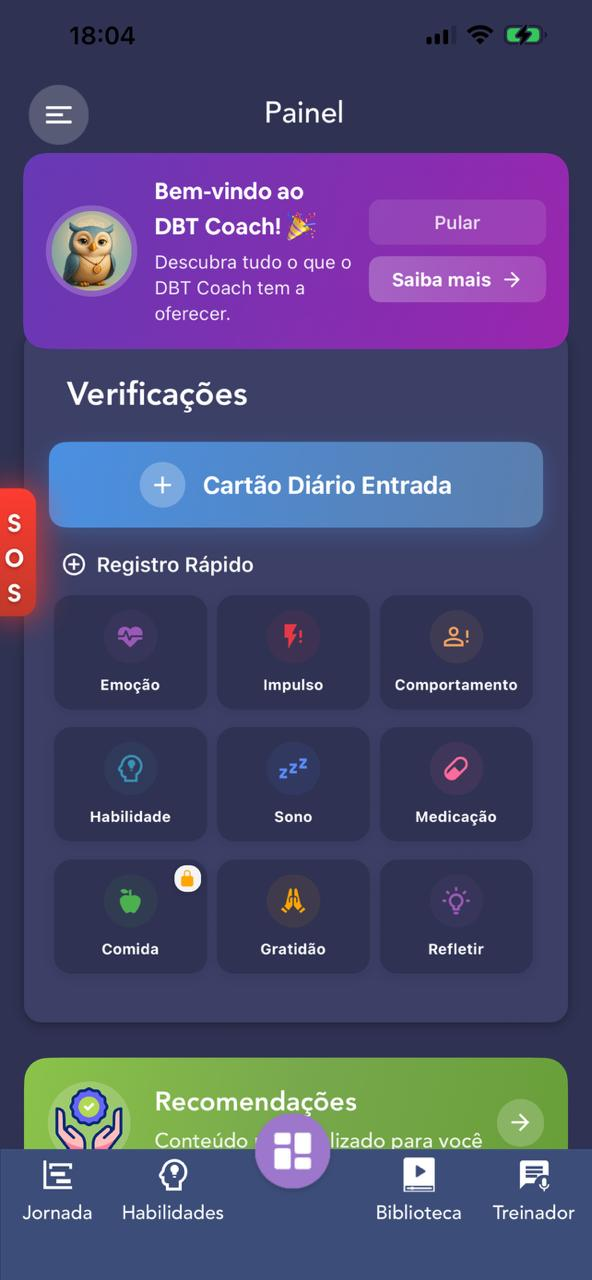
\includegraphics[height=9cm, keepaspectratio]{dados/figuras/telaDBTCoach_1} 
        \centerline{\small (a) Interface de registros} % <-- Subtítulo A
    \end{minipage}\hfill
    % --- Imagem B ---
    \begin{minipage}[b]{0.46\textwidth}
        \centering
        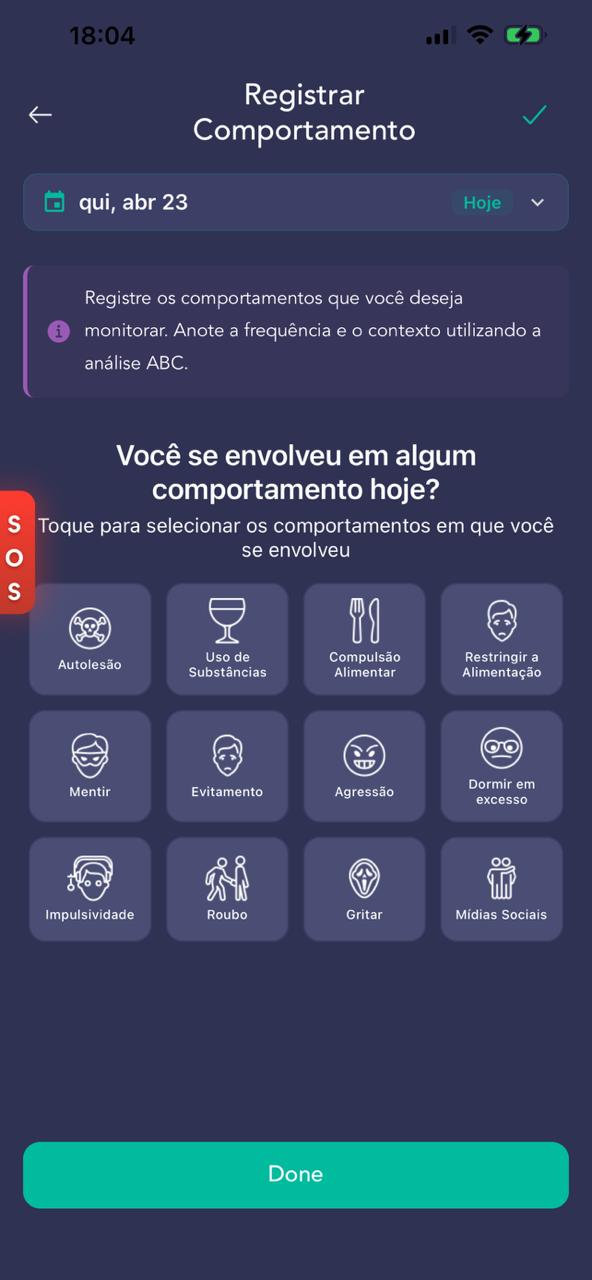
\includegraphics[height=9cm, keepaspectratio]{dados/figuras/telaDBTCoach_2}
        \centerline{\small (b) Painel clínico} % <-- Subtítulo B
    \end{minipage}
    
   \vspace{0.3cm}
    \begin{flushleft} % <-- Inicia o alinhamento à esquerda
        \footnotesize Fonte: DBT Coach (2026) % <-- Sem o \legend, apenas o texto!
    \end{flushleft}   
\end{figure}

\vspace{0.3cm}
\subsection{ClassDojo}

O ClassDojo é uma plataforma de gestão escolar e comunicação disponível via web e em aplicativos móveis, amplamente utilizada para conectar a escola à família \cite{classdojo2026}. O software tem como propósito central a gamificação do comportamento em sala de aula e a criação de uma comunidade escolar integrada. Seu público-alvo principal são professores da educação básica, alunos e seus respectivos responsáveis.

O software permite a criação de turmas digitais onde cada aluno é representado por um avatar personalizável. As principais funcionalidades incluem o compartilhamento de fotos e vídeos das atividades e um sistema de atribuição de pontos. Os professores podem configurar competências positivas ou pontos a melhorar, emitindo relatórios automáticos sobre o engajamento dos estudantes. O aplicativo ainda permite a troca de mensagens diretas e privadas entre a escola e os pais.

A interface do aplicativo aposta em um design lúdico e colorido para atrair o público infantil. Conforme ilustrado na Figura 2.2, a tela de gestão da turma apresenta avatares em formato de monstrinhos que mudam conforme a pontuação recebida. Ao selecionar um aluno, o sistema abre um menu flutuante com ícones verdes para reforços positivos (como "Trabalho duro") e ícones vermelhos com sinal de menos (-1) para comportamentos que precisam de ajuste (como "Falta de foco"), oferecendo um feedback visual imediato sobre a conduta do estudante.
\begin{figure}[H] 
    \centering
    \caption{Telas principais do aplicativo ClassDojo} % <-- Legenda ÚNICA no topo
    \label{fig:telas_dbt}
    \vspace{0.3cm}
    
    % --- Imagem A ---
    \begin{minipage}[b]{0.46\textwidth}
        \centering
        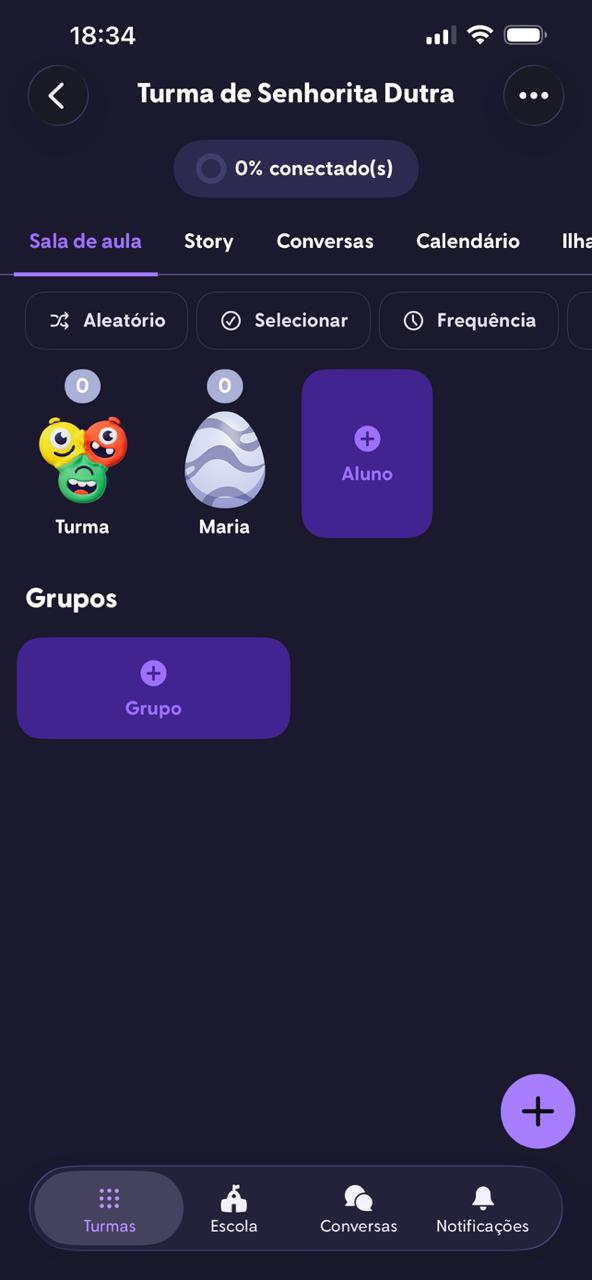
\includegraphics[height=9cm, keepaspectratio]{dados/figuras/telaClassDojo_1} 
        \centerline{\small (a) Visão geral da turma} % <-- Subtítulo A
    \end{minipage}\hfill
    % --- Imagem B ---
    \begin{minipage}[b]{0.46\textwidth}
        \centering
        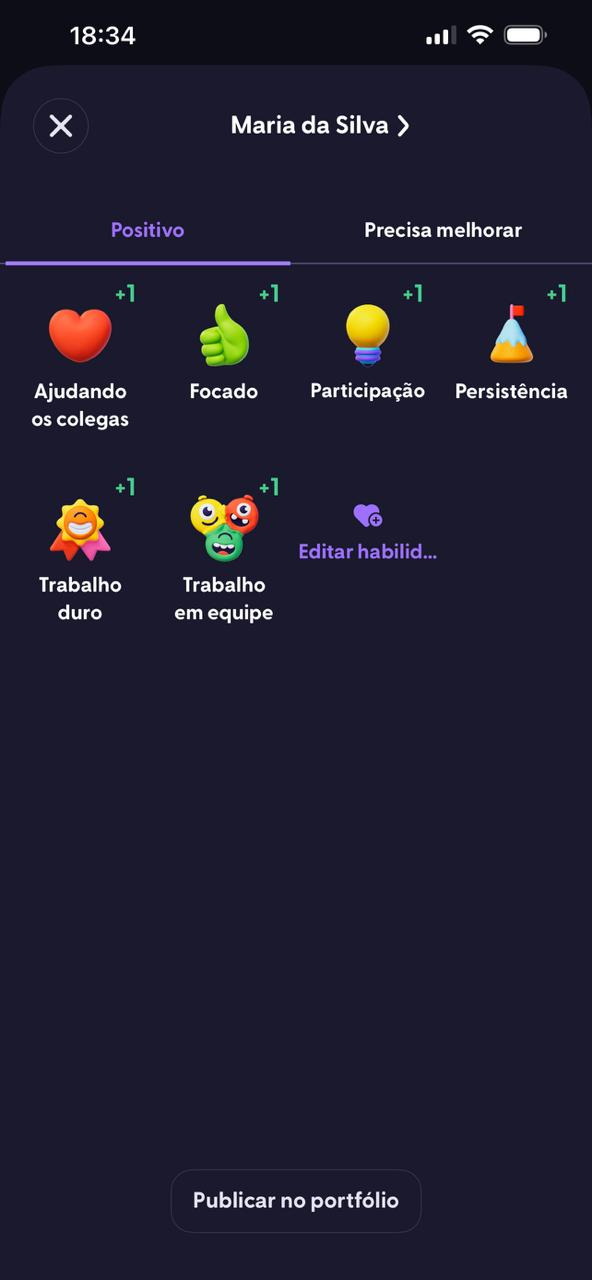
\includegraphics[height=9cm, keepaspectratio]{dados/figuras/telaClassDojo_2}
        \centerline{\small (b) Interface de pontuações} % <-- Subtítulo B
    \end{minipage}
    
    \vspace{0.3cm}
    \begin{flushleft} % <-- Inicia o alinhamento à esquerda
    \footnotesize{Fonte: ClassDojo (2026)} % <-- Fonte ÚNICA no final
 \end{flushleft}   
\end{figure}

\vspace{0.2cm}

Contudo, o sistema apresenta falhas metodológicas quando aplicado ao público com TDAH e TOD. O modelo de gamificação baseada em punição pública (perda de pontos visível) pode gerar ansiedade e reforçar o comportamento opositor. Adicionalmente, as avaliações de usuários indicam que o software falha ao não permitir o registro detalhado e privado de ocorrências comportamentais complexas, transformando a comunicação em uma linha do tempo genérica que não orienta os pais sobre como intervir tecnicamente em casa. 

\vspace{0.3cm}
\subsection{Pictalk Buddy}
 
 O Pictalk Buddy é um aplicativo de tecnologia assistiva disponível para smartphones, desenvolvido por uma organização focada em acessibilidade cognitiva \cite{pictalk2026}. O software permite a criação de agendas visuais para auxiliar pessoas com dificuldades na função executiva. Seu público-alvo compreende crianças e adultos com TEA, TDAH e outras condições que se beneficiam da previsibilidade das tarefas diárias.

O software permite a criação passo a passo das rotinas por meio de pictogramas e recursos de voz. As principais funcionalidades envolvem a organização sequencial de atividades, onde o aplicativo gera alertas sonoros que lembram o usuário sobre cada etapa a ser realizada. O sistema também oferece suporte para comunicação alternativa, permitindo que o usuário expresse necessidades básicas através de imagens caso encontre dificuldades na fala verbal.

A usabilidade do Pictalk Buddy é pautada na clareza visual e no minimalismo para evitar a sobrecarga sensorial. Conforme ilustrado na Figura 2.3, a interface é composta por grandes cartões quadrados que contêm ilustrações simples de tarefas cotidianas, como "Escovar os dentes" ou "Lanche". Abaixo de cada imagem, há uma legenda em texto e um botão de áudio; ao ser tocado, o aplicativo narra a instrução em voz alta, permitindo que o usuário avance na rotina de forma autônoma e acompanhe visualmente o progresso do seu dia.
\begin{figure}[H] 
    \centering
    \caption{Telas principais do aplicativo PicTalk} % <-- Legenda ÚNICA no topo
    \label{fig:telas_dbt}
    \vspace{0.3cm}
    
    % --- Imagem A ---
    \begin{minipage}[b]{0.46\textwidth}
        \centering
        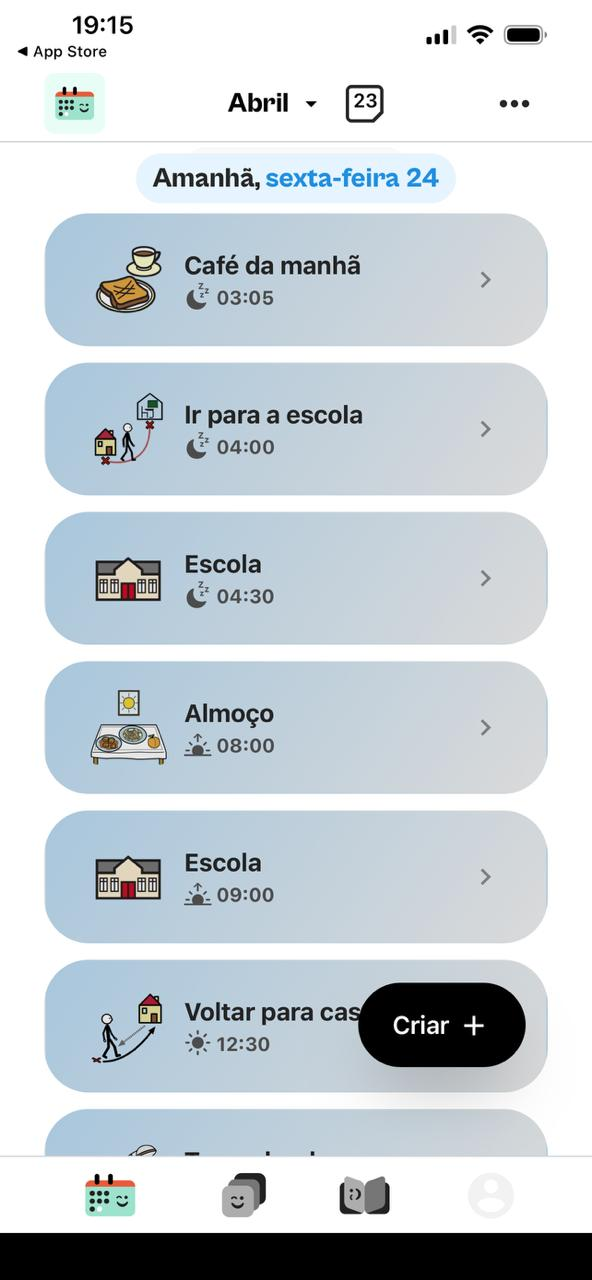
\includegraphics[height=9cm, keepaspectratio]{dados/figuras/telaPicTalk_1} 
        \centerline{\small (a) Agenda visual no aplicativo} % <-- Subtítulo A
    \end{minipage}\hfill
    % --- Imagem B ---
    \begin{minipage}[b]{0.46\textwidth}
        \centering
        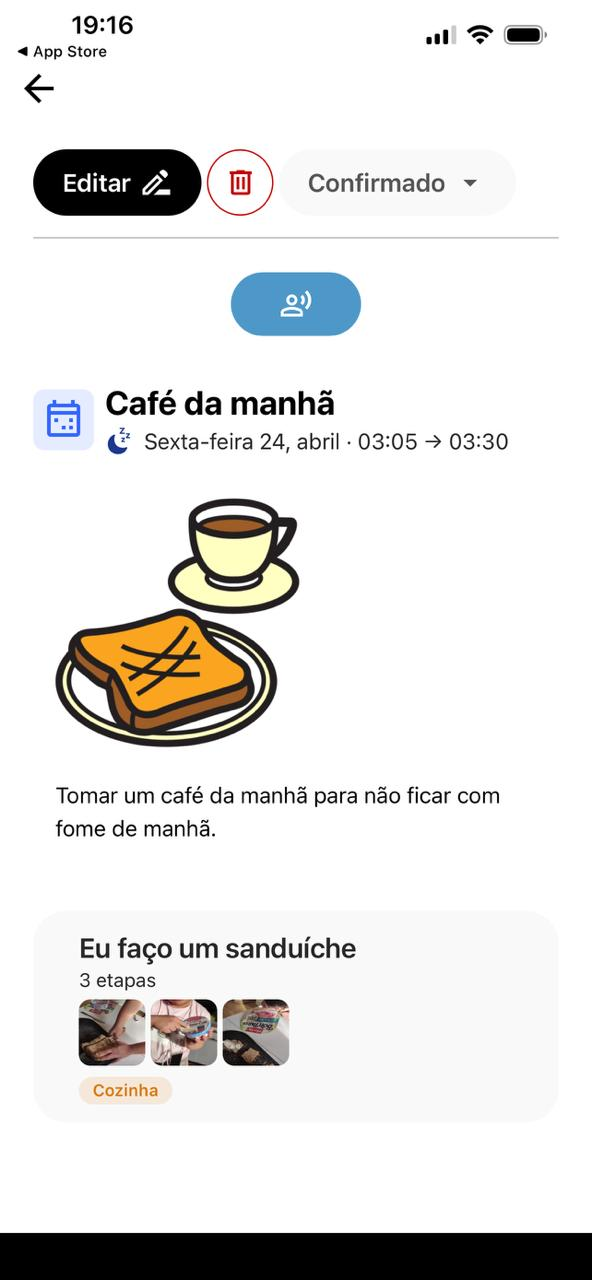
\includegraphics[height=9cm, keepaspectratio]{dados/figuras/telaPicTalk_2}
        \centerline{\small (b) Organização de agenda de café da manhã} % <-- Subtítulo B
    \end{minipage}
    
  \vspace{0.3cm}
    \begin{flushleft} % <-- Inicia o alinhamento à esquerda
   \footnotesize{Fonte: PicTalk (2026)} % <-- Fonte ÚNICA no final
 \end{flushleft}   
\end{figure}

\vspace{0.2cm}
Apesar de ser eficaz na promoção da autonomia individual, a ferramenta não supre as necessidades de uma gestão escolar compartilhada. Por ser um aplicativo pago e focado no uso pessoal da criança, ele não oferece recursos para que o professor registre comportamentos desafiadores ou alinhe estratégias táticas com os pais. O software atua na prevenção por meio da rotina, mas falha em prover um canal de comunicação e suporte para o manejo comportamental reativo necessário no contexto do TDAH e do TOD.

\vspace{0.3cm}
\subsection{Sequência Mágica}

O sistema web "Sequência Mágica", desenvolvido como pesquisa acadêmica no Instituto Federal de Brasília \cite{santos2025}, é uma plataforma interativa voltada para a organização de rotinas. O propósito principal da ferramenta é auxiliar no desenvolvimento da autonomia e do raciocínio lógico por meio da estruturação de atividades cotidianas. Seu público-alvo direto compreende crianças de 2 a 4 anos diagnosticadas com Transtorno do Espectro Autista (TEA), bem como educadores da primeira infância e pais que auxiliam na mediação dessas atividades.

As principais funcionalidades do sistema baseiam-se na criação interativa de sequências visuais. A plataforma permite que o usuário selecione blocos representativos de ações do dia a dia (como "acordar", "tomar banho" e "escovar os dentes") e os posicione na ordem correta utilizando o recurso de arrastar e soltar (drag and drop). Além disso, o software possui recursos para salvar a rotina montada no armazenamento local do navegador (localStorage), permitindo a visualização, restauração ou exclusão de sequências previamente configuradas e associadas à data atual.

A Figura 2.4 apresenta as telas principais do protótipo do sistema Sequência Mágica. Em relação à usabilidade, o aplicativo adota uma interface voltada para a acessibilidade cognitiva do público infantil, priorizando a clareza visual e a simplicidade de navegação. Como pode ser observado na tela de início (a), há o uso de personagens lúdicos e cores suaves que geram empatia imediata. Já na tela de montagem da sequência (b), a estruturação utiliza uma barra lateral com blocos de rotina diária (como acordar e tomar banho), representados por pictogramas coloridos e legendas simples. Essa disposição limpa e interativa no painel principal permite que a criança acompanhe e estruture o seu próprio dia de forma intuitiva, promovendo a previsibilidade e evitando a sobrecarga sensorial.
\begin{figure}[H] 
    \centering
    \caption{Telas principais do protótipo de Sequência Mágica} % <-- Legenda ÚNICA no topo
    \label{fig:telas_dbt}
    \vspace{0.3cm}
    
    % --- Imagem A ---
    \begin{minipage}[b]{0.46\textwidth}
        \centering
        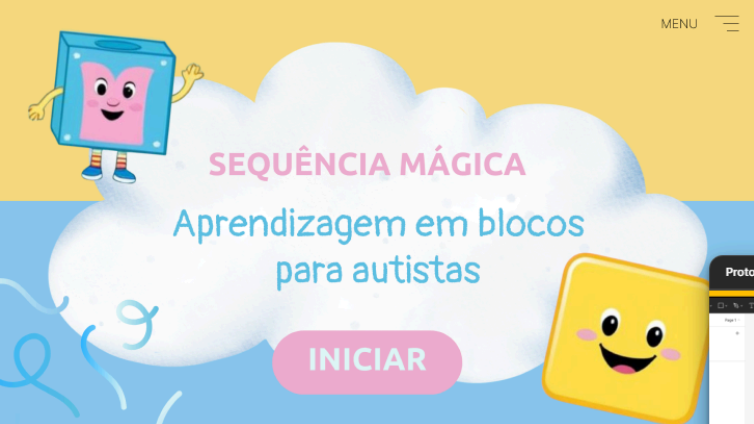
\includegraphics[height=9cm, keepaspectratio]{dados/figuras/telaSequenciaMagica_1} 
        \centerline{\small (a) Tela de início} % <-- Subtítulo A
    \end{minipage}\hfill
    % --- Imagem B ---
    \begin{minipage}[b]{0.46\textwidth}
        \centering
        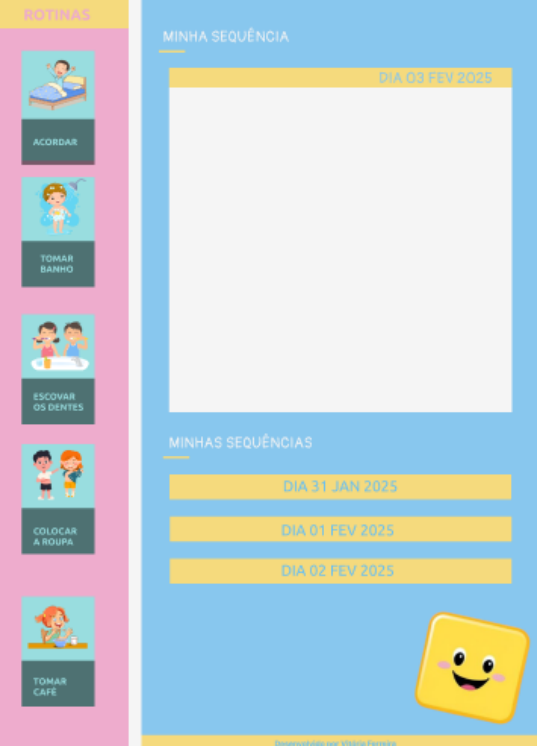
\includegraphics[height=9cm, keepaspectratio]{dados/figuras/telaSequenciaMagica_2}
        \centerline{\small (b)  Tela de montagem da sequência dos cards} % <-- Subtítulo B
    \end{minipage}
    
   \vspace{0.3cm}
    \begin{flushleft} % <-- Inicia o alinhamento à esquerda
   \footnotesize{Fonte: Silva (2025, p. 30, 31).} % <-- Fonte ÚNICA no final
 \end{flushleft}   
\end{figure}

\vspace{0.2cm}
Apesar de ser uma iniciativa acadêmica de excelência para a educação infantil, a plataforma apresenta limitações metodológicas e técnicas frente aos objetivos deste projeto. O primeiro obstáculo é estrutural: por utilizar o armazenamento local (localStorage) e não possuir sistema de autenticação ou banco de dados em nuvem, o aplicativo restringe os dados a um único dispositivo, impedindo o compartilhamento de informações integradas entre a escola e a família. Ademais, por focar estritamente na organização preventiva de rotinas para crianças de 2 a 4 anos, a ferramenta não contempla um módulo de comunicação escolar, registro de ocorrências ou suporte tático para o manejo reativo de crises associadas ao TDAH e ao TOD no ambiente educacional.
\vspace{0.3cm}

\section{Análise Comparativa}

Após a análise individual das ferramentas, o Quadro \ref{quadro:comparativo_sistemas} apresenta uma síntese comparativa. Fica evidente que, embora existam soluções robustas para a comunicação alternativa (PicTalk), gamificação (ClassDojo) ou rotinas diárias (Sequência Mágica), há uma lacuna no que diz respeito a um sistema escolar que integre o registro de ocorrências à oferta ativa de estratégias de manejo para professores de alunos com TDAH e TOD, necessidade esta que a solução proposta visa suprir.

\begin{table}[H]
    \centering
    \caption{Comparativo entre os sistemas similares e a solução proposta}
    \label{quadro:comparativo_sistemas}
    \renewcommand{\arraystretch}{1.4} 
    \setlength{\tabcolsep}{3pt}
    \small 

    \begin{tabular}{|p{2.4cm}|p{3.8cm}|p{2.5cm}|p{2.4cm}|p{2.0cm}|p{1.8cm}|}
        \hline
        \textbf{Sistema} & \textbf{Foco Principal} & \textbf{Público-Alvo} & \textbf{Comunicação \newline Escola-Família} & \textbf{Sugestões \newline de Manejo} & \textbf{Plataforma} \\ \hline
        
        \textbf{DBT Coach} & Regulação emocional e habilidades de enfrentamento clínico. & Pacientes e terapeutas & Não & Sim (Clínico) & App Mobile \\ \hline
        
        \textbf{ClassDojo} & Gestão de sala de aula, engajamento e gamificação de comportamento. & Professores, pais e alunos & Sim & Não & Web e Mobile \\ \hline
        
        \textbf{PicTalk} & Comunicação Alternativa e Aumentativa (CAA) com pictogramas. & Crianças, pais e terapeutas & Não & Não & App Mobile \\ \hline
        
        \textbf{Sequência Mágica} & Organização de rotinas diárias e acessibilidade cognitiva. & Crianças e pais & Não & Não & App Mobile \\ \hline
        
        \textbf{Sistema Proposto} & Registro comportamental contínuo e suporte estratégico pedagógico. & Professores e pais \newline (Foco em TDAH/TOD) & Sim & Sim & Web Resp. \\ \hline
    \end{tabular}
    
    \vspace{0.2cm}
    \legend{Fonte: Elaborado pelo autor (2026)}
\end{table}

\vspace{0.3cm}
\section{Considerações do Capítulo}

Este capítulo apresentou os principais sistemas e conceitos que fundamentam a pesquisa, abordando ferramentas voltadas ao manejo do Transtorno de Déficit de Atenção com Hiperatividade (TDAH) e do Transtorno Opositor Desafiador (TOD), bem como plataformas de comunicação escolar e tecnologias de regulação emocional. A análise comparativa desses recursos forneceu a base necessária para a compreensão das necessidades da rede de apoio (escola e família) e evidenciou a lacuna tecnológica existente no mercado, justificando e sustentando o desenvolvimento da proposta apresentada nos capítulos seguintes.           % Fundamentação teórica
    % ----------------------------------------------------------------------------
%                                  METODOLOGIA
% ----------------------------------------------------------------------------

\chapter{METODOLOGIA}
\label{chap:metodologia}

Este capítulo descreve os procedimentos metodológicos e técnicos adotados para a concepção, o desenvolvimento e a validação do sistema proposto. O objetivo é detalhar o percurso percorrido desde a identificação do problema até a estruturação da solução tecnológica voltada para o manejo comportamental e a comunicação escolar de alunos com TDAH e TOD. Para isso, são apresentados a classificação da pesquisa, o modelo de engenharia de software escolhido, as técnicas de levantamento de requisitos e as tecnologias utilizadas na construção da plataforma.

\vspace{0.5cm}
\section{Descrição Geral da Pesquisa}

A pesquisa delineada neste projeto classifica-se, quanto à sua natureza, como aplicada, visto que busca gerar conhecimentos para aplicação prática na resolução de problemas de comunicação entre família e escola no cenário da neurodivergência. Segundo \citeonline{prodanov2013}, a pesquisa aplicada caracteriza-se pelo interesse na aplicação e nas consequências práticas do conhecimento.

Em relação aos objetivos, trata-se de um estudo de caráter exploratório que, conforme define \citeonline{gil2002}, visa desenvolver e esclarecer conceitos para proporcionar uma visão geral sobre um determinado fato. Neste trabalho, a etapa exploratória consolida-se através da revisão bibliográfica e da análise de sistemas similares, fundamentais para mapear as lacunas tecnológicas do mercado educacional.

Por fim, a abordagem metodológica é qualitativa. O foco central não reside na quantificação de variáveis numéricas, mas na compreensão detalhada da dinâmica escolar e familiar, permitindo a correta tradução das necessidades pedagógicas e de manejo comportamental em requisitos de software.

Cabe ressaltar que, devido às restrições temporais inerentes ao desenvolvimento deste trabalho, o escopo desta publicação delimitou-se à concepção, especificação técnica e prototipagem de alta fidelidade da aplicação web responsiva, não englobando as fases de implementação do código-fonte e testes empíricos com usuários. Contudo, com o intuito de garantir a continuidade e a futura validação prática da solução proposta, foi firmada uma articulação institucional para que o sistema seja submetido a um estudo de caso em ambiente real no Instituto Federal de Brasília (IFB). Essa etapa futura viabilizará a análise do impacto gerado pelos cards de manejo proativo diretamente na rotina dos docentes e na comunicação com os familiares das crianças neurodivergentes.

\vspace{0.5cm}
\section{3.2 Instrumentos de Pesquisa}

    Para o levantamento de requisitos e a compreensão aprofundada do contexto escolar e
familiar de alunos com 
TDAH e TOD, o presente estudo apoia-se em instrumentos metodológicos diversificados. A escolha dessas 
ferramentas fundamenta-se na necessidade de captar as percepções dos usuários, observar a dinâmica do ambiente 
educacional e validar a solução tecnológica proposta. Os instrumentos definidos para esta pesquisa são:
\vspace{0.3cm}

No contexto deste trabalho, as entrevistas semiestruturadas, fundamentadas em \citeonline{gil2002}, permitiram explorar de maneira flexível as percepções dos participantes, combinando perguntas abertas com tópicos previamente definidos. Isso favoreceu respostas detalhadas e espontâneas, sendo essenciais para captar as necessidades comunicativas e as expectativas de familiares e educadores em relação ao manejo comportamental. Além disso, a observação participante e as visitas em campo viabilizaram a análise do comportamento dos sujeitos em seu ambiente natural, registrando interações e padrões cotidianos \citeonline{creswell2014}. Esse instrumento foi fundamental para entender a dinâmica real da sala de aula, as estratégias já utilizadas pelos professores e as reações espontâneas no suporte às neurodivergências.

Paralelamente a isso, a aplicação de um questionário online, estruturado com questões abertas e fechadas via Google Forms, atuou como um recurso decisivo para mapear as necessidades técnicas e as expectativas dos usuários. A coleta de dados através desse questionário permitiu identificar não apenas as demandas gerais, mas também as principais "dores" e limitações enfrentadas pelos docentes no seu cotidiano. A análise das respostas revelou dois pontos cruciais que redefiniram o escopo do projeto.

Em primeiro lugar, os educadores manifestaram a preocupação de que a plataforma pudesse tornar-se apenas mais um meio de registro passivo, funcionando como uma versão digital do tradicional "livro de atas" ou diário de turma, onde os acontecimentos são documentados, mas sem a oferta de soluções práticas. Para mitigar esta questão, definiu-se que o sistema deveria assumir uma postura proativa, fornecendo sugestões, exemplos de manejo comportamental e estratégias de intervenção baseadas em evidências para auxiliar no suporte a alunos com TDAH e TOD.

Em segundo lugar, o levantamento expôs um obstáculo infraestrutural: a recusa de alguns docentes em utilizar os seus celulares e redes de dados pessoais para o trabalho escolar. No entanto, constatou-se que as escolas estão equipadas com computadores para uso institucional. Para contornar essa limitação técnica e garantir a adesão ao sistema, decidiu-se que o projeto seria desenvolvido sob a arquitetura de uma Aplicação Web Responsiva. Esta abordagem permite que a plataforma seja acessada diretamente através de um navegador \textit{(browser)} em qualquer computador da escola, sem a necessidade de instalar aplicativos. Em simultâneo, a responsividade garante que a interface se adapte de forma automática e otimizada às telas dos celulares dos pais, permitindo-lhes acompanhar as ocorrências com total mobilidade.

Portanto, diante dessas definições, avançou-se para a prototipagem de alta fidelidade. A interface desenvolvida (construída no Figma) atuará como um instrumento visual de validação, permitindo que os usuários visualizem as funcionalidades propostas e forneçam \textit{feedbacks} iniciais sobre a usabilidade, a clareza visual e a acessibilidade cognitiva do sistema.

\vspace{0.5cm}
\section{Coleta e Análise de Dados}

Nesta etapa, define-se como os dados coletados pelos instrumentos de pesquisa serão processados e interpretados, a partir do uso experimental e da validação dos protótipos do sistema nas dependências do Instituto Federal de Brasília. Durante as sessões de apresentação da ferramenta, serão registradas as reações espontâneas dos educadores e familiares, possíveis dificuldades de navegação na interface web, preferências de layout e o nível de compreensão das funcionalidades propostas. As entrevistas semiestruturadas complementarão esses dados, fornecendo impressões detalhadas dos professores e responsáveis sobre a utilidade da plataforma no cotidiano.

As sessões de observação e as visitas em campo permitirão acompanhar a dinâmica escolar em tempo real, registrando os comportamentos, as estratégias de interação adotadas pelos docentes no manejo do TDAH e do TOD, e as possíveis dificuldades enfrentadas no registro tradicional de ocorrências.

O volume de dados qualitativos obtidos (transcrições de entrevistas e anotações de campo) será organizado e interpretado por meio da Análise de Conteúdo \citeonline{bardin2011}. Esse método permitirá a identificação de categorias temáticas, padrões de comportamento, gargalos na comunicação escola-família e aspectos cruciais de usabilidade. Essa abordagem estruturada possibilitará avaliar a eficácia conceitual do aplicativo web, fornecendo subsídios e métricas concretas para o refinamento contínuo da ferramenta e a consolidação dos requisitos do software.  
    % Metodologia
    \include{estrutura/textuais/desenvolvimento/resultados}              % Resultados
    % ----------------------------------------------------------------------------
%                             Proposta de Desenvolvimento
% ----------------------------------------------------------------------------
\chapter{Proposta}
\label{chap:proposta}

\vspace{0.2cm}
\section{Cronograma}

O Quadro 1 apresenta o cronograma do trabalho, que ilustra as etapas fundamentais do desenvolvimento e da pesquisa distribuídas ao longo dos dois semestres letivos de 2026. Cada etapa planeada visa garantir a realização estruturada e eficiente das atividades, culminando na conclusão e defesa do trabalho final.

\vspace{0.2cm}
\noindent O planeamento está dividido em quatro fases principais:

\begin{enumerate}
    \item \textbf{Fase de Estruturação e Fundamentação (Fev/26 a Abr/26):} Inclui a definição do tema, delimitação do problema e o levantamento bibliográfico sobre TDAH e TOD. Nesta fase também foi realizado o levantamento de requisitos com os educadores para subsidiar a construção do sistema.

    \item \textbf{Fase de Design e Prototipação (Abr/26 a Jun/26):} Abrange o planeamento visual da solução em formato Web Responsivo, com foco na criação dos ecrãs no Figma para definir a Interface de Utilizador (UI/UX). Esta etapa contempla a redação do Pré-TCC e a sua apresentação.

    \item \textbf{Fase de Desenvolvimento e Validação (Ago/26 a Out/26):} Envolve a implementação do sistema em código (React.js), a configuração da base de dados em nuvem (Firebase) e a realização de testes de usabilidade e funcionamento do software.

    \item \textbf{Fase de Finalização e Entrega (Out/26 a Dez/26):} Foca-se nos ajustes finais do sistema após a fase de testes. Esta etapa inclui a redação final do TCC, a formatação nas normas ABNT e culmina com a Apresentação e Defesa Final do Trabalho.
\end{enumerate}

\begin{table}[H]
\centering
\caption{Cronograma de atividades do TCC (2026)}
\label{quadro:cronograma}
\renewcommand{\arraystretch}{1.3} 
\setlength{\tabcolsep}{4pt} 
\small 
\begin{tabular}{|p{4.5cm}|c|c|c|c|c|c|c|c|c|c|}
\hline

\multicolumn{1}{|c|}{\textbf{Etapas do Projeto}} & \multicolumn{10}{c|}{\textbf{Período (Mês)}} \\ \cline{2-11} 
 & \textbf{fev} & \textbf{mar} & \textbf{abr} & \textbf{mai} & \textbf{jun} & \textbf{ago} & \textbf{set} & \textbf{out} & \textbf{nov} & \textbf{dez} \\ \hline

Escolha do tema e delimitação do problema & X & & & & & & & & & \\ \hline
Levantamento bibliográfico e sistemas similares & X & X & & & & & & & & \\ \hline
Levantamento e análise de requisitos & & X & X & & & & & & & \\ \hline
Planeamento e prototipação das telas no Figma & & & X & X & & & & & & \\ \hline
Redação parcial do TCC (Metodologia e Cap. Iniciais) & & & X & X & & & & & & \\ \hline
Revisão com o orientador e formatação & X & X & X & X & X & X & X & X & X & X \\ \hline
Apresentação do Pré-TCC & & & & & X & & & & & \\ \hline
Configuração da Base de Dados (Firebase) & & & & & & X & & & & \\ \hline
Implementação do sistema web responsivo (React) & & & & & & X & X & X & & \\ \hline
Testes de funcionalidade e ajustes & & & & & & & & X & X & \\ \hline
Redação final do TCC (Resultados e Conclusão) & & & & & & & & X & X & \\ \hline
Revisão final, preparação e ensaio da apresentação & & & & & & & & & X & \\ \hline
Apresentação final do TCC & & & & & & & & & & X \\ \hline
\end{tabular}

\vspace{0.2cm}
\legend{Fonte: Elaborado pelo autor (2026)}
\end{table}

\section{Requisitos de Usuário (RU)}

Os requisitos de usuário foram elaborados visando o acompanhamento adequado dos alunos com TDAH e TOD, levando em conta o suporte oferecido por professores e responsáveis durante a utilização da plataforma web.

\vspace{0.3cm}
RU01 - Organização das Salas: Como educador, eu preciso criar e estruturar minhas turmas de forma virtual, vinculando os respectivos alunos, para que a gestão dos perfis seja iniciada de maneira correta no sistema. 

RU02 - Visão Rápida da Turma: Como educador, eu desejo visualizar todos os meus alunos em um painel \textit{(dashboard)} claro e organizado no computador da escola, para que eu possa iniciar o meu dia letivo e localizar rapidamente o perfil de um aluno específico.

RU03 - Agilidade no Registro de Crises: Como educador, eu preciso conseguir registrar uma ocorrência comportamental de forma muito rápida, utilizando botões e tags predefinidas em vez de digitar textos longos, para que eu não perca o controle da turma nem me sobrecarregue durante o manejo de um momento de agitação.

RU04 - Suporte Pedagógico Imediato: Como educador, eu desejo receber sugestões práticas de manejo e intervenção assim que eu registrar um comportamento desafiador, para que a plataforma atue como um apoio real em sala de aula, e não apenas como um diário de registros passivo.

RU05 - Histórico Compartilhado: Como educador e familiar, eu preciso ter acesso a um histórico consolidado de ocorrências passadas, para que eu possa identificar padrões de gatilhos comportamentais ao longo do tempo.

RU06 - Acompanhamento Transparente e Móvel: Como familiar, eu desejo acompanhar a rotina e as ocorrências do meu filho através de uma linha do tempo \textit{(timeline)} acessível pelo meu celular, para que eu tenha ciência imediata das estratégias aplicadas na escola e possa dar continuidade a elas em casa, evitando conflitos de comunicação.

RU07 - Relatórios para Apoio Clínico: Como educador e familiar, eu preciso gerar relatórios visuais de evolução comportamental, para que eu possa compartilhar esses dados concretos com a equipe médica e terapêutica do aluno (neuropediatras e psicólogos), auxiliando no ajuste de intervenções e medicamentos.

RU08 - Privacidade e Acesso Focado: Como familiar, eu preciso acessar o sistema de forma segura e visualizar apenas as informações referentes ao meu filho, para garantir a privacidade dos dados sensíveis e o cumprimento das normas de proteção à criança (ECA e LGPD \cite{lei13709_2018, lei8069_1990}).

RU09 - Autonomia no Cadastro: Como novo usuário, eu desejo realizar o meu próprio cadastro na plataforma de forma simples, identificando-me como educador ou familiar, para obter credenciais de acesso válidas no sistema.

\vspace{0.5cm}
\section{Requisitos Funcionais (RF)}

Os requisitos funcionais descrevem as operações e funcionalidades essenciais do sistema, garantindo a interação eficiente entre os usuários e a aplicação web.

\begin{quadro}[H]
    \centering
    \caption{Quadro de Requisitos Funcionais do Sistema}
    \label{quadro:requisitos_funcionais}
    \renewcommand{\arraystretch}{1.5} % Aumenta o espaçamento interno das linhas
    \small % Ajusta a fonte para caber confortavelmente nas margens
    
    \begin{tabular}{|c|p{4cm}|p{7.5cm}|c|}
        \hline
        \textbf{Código} & \textbf{Requisito Funcional} & \textbf{Descrição} & \textbf{Caso de Uso} \\ \hline
        
        \textbf{RF01} & Estruturar Turmas & O sistema deve permitir que o educador crie e organize turmas virtuais, vinculando os respectivos alunos ao seu painel. & UC01 \\ \hline
        
        \textbf{RF02} & Exibir Painel Geral & O sistema deve apresentar um \textit{dashboard} com a listagem visual e o estado atualizado de todos os alunos da turma selecionada. & UC02 \\ \hline
        
        \textbf{RF03} & Registrar Ocorrências & O sistema deve permitir que o educador registre comportamentos e crises de forma ágil, utilizando categorias predefinidas (\textit{chips/tags}). & UC03 \\ \hline
        
        \textbf{RF04} & Visualizar Sugestões de Manejo & O sistema deve exibir automaticamente \textit{cards} com estratégias de intervenção proativa logo após o registro de uma ocorrência. & UC04 \\ \hline
        
        \textbf{RF05} & Consultar Histórico & O sistema deve permitir que educadores e familiares visualizem o detalhamento de ocorrências e eventos passados do aluno. & UC05 \\ \hline
        
        \textbf{RF06} & Acompanhar Linha do Tempo & O sistema deve disponibilizar um \textit{feed} cronológico (\textit{timeline}) para que o familiar acompanhe a rotina diária e os registros do aluno. & UC06 \\ \hline
        
        \textbf{RF07} & Emitir Relatórios & O sistema deve compilar os dados comportamentais e gerar relatórios consolidados e exportáveis (PDF) para apoio clínico. & UC07 \\ \hline
        
        \textbf{RF08} & Autenticar no Sistema & O sistema deve validar o acesso de educadores e familiares por meio da inserção de credenciais seguras (e-mail e senha). & UC08 \\ \hline
        
        \textbf{RF09} & Cadastrar Usuário & O sistema deve permitir a criação de novas contas, vinculando os dados de identificação ao perfil correto (Educador ou Familiar). & UC09 \\ \hline
    \end{tabular}
    
    \vspace{0.1cm}
    \begin{flushleft}
        \footnotesize Fonte: Elaborada pela autora (2026).
    \end{flushleft}
\end{quadro}

\vspace{0.1cm}
\section{Requisitos Não Funcionais (RFN)}

Os requisitos não funcionais especificam os critérios de qualidade e as restrições arquitetónicas da plataforma:

% --- RNF01 ---
\begin{quadro}[H]
    \centering
    \caption{RNF01: Arquitetura Web Responsiva}
    \label{quadro:rnf01}
    \renewcommand{\arraystretch}{1.5}
    \begin{tabular}{|p{5.5cm}|p{2.5cm}|p{7cm}|}
        \hline
        \multicolumn{3}{|c|}{\textbf{RNF01 - Arquitetura Web Responsiva}} \\ \hline
        \textbf{Descrição} & \textbf{Categoria} & \textbf{RU Atendido} \\ \hline
        Relação \textit{Mobile-First} adaptável de forma automática a computadores e celulares. & Portabilidade & \textbf{RU02 e RU05:} Permite que docentes usem os computadores da escola e os pais usem seus smartphones, sem necessidade de instalação. \\ \hline
    \end{tabular}
    
    \vspace{0.1cm}
    \begin{flushleft}
        \footnotesize Fonte: Elaborada pela autora (2026).
    \end{flushleft}
\end{quadro}

% --- RNF02 ---
\begin{quadro}[H]
    \centering
    \caption{RNF02: Acessibilidade Cognitiva}
    \label{quadro:rnf02}
    \renewcommand{\arraystretch}{1.5}
    \begin{tabular}{|p{5.5cm}|p{2.5cm}|p{7cm}|}
        \hline
        \multicolumn{3}{|c|}{\textbf{RNF02 - Acessibilidade Cognitiva}} \\ \hline
        \textbf{Descrição} & \textbf{Categoria} & \textbf{RU Atendido} \\ \hline
        Interface limpa, cores suaves, fontes sem serifa e fluxos curtos (poucos cliques). & Usabilidade & \textbf{RU03:} Evita a sobrecarga sensorial e o estresse do professor, facilitando o uso rápido mesmo em momentos de crise na sala. \\ \hline
    \end{tabular}
    
    \vspace{0.1cm}
    \begin{flushleft}
        \footnotesize Fonte: Elaborada pela autora (2026).
    \end{flushleft}
\end{quadro}

% --- RNF03 ---
\begin{quadro}[H]
    \centering
    \caption{RNF03: Tempo de Resposta}
    \label{quadro:rnf03}
    \renewcommand{\arraystretch}{1.5}
    \begin{tabular}{|p{5.5cm}|p{2.5cm}|p{7cm}|}
        \hline
        \multicolumn{3}{|c|}{\textbf{RNF03 - Tempo de Resposta}} \\ \hline
        \textbf{Descrição} & \textbf{Categoria} & \textbf{RU Atendido} \\ \hline
        Processamento de registros e exibição de sugestões em no máximo 3 segundos. & Desempenho & \textbf{RU03 e RU04:} Garante que o \textit{software} responda em tempo real, impedindo que o professor perca o foco na turma devido a travamentos. \\ \hline
    \end{tabular}
    
    \vspace{0.1cm}
    \begin{flushleft}
        \footnotesize Fonte: Elaborada pela autora (2026).
    \end{flushleft}
\end{quadro}

% --- RNF04 ---
\begin{quadro}[H]
    \centering
    \caption{RNF04: Segurança, Privacidade e Controle de Acesso}
    \label{quadro:rnf04}
    \renewcommand{\arraystretch}{1.5}
    \begin{tabular}{|p{5.5cm}|p{2.5cm}|p{7cm}|}
        \hline
        \multicolumn{3}{|c|}{\textbf{RNF04 - Segurança, Privacidade e Controle de Acesso}} \\ \hline
        \textbf{Descrição} & \textbf{Categoria} & \textbf{RU Atendido} \\ \hline
        O sistema deve restringir a visualização de dados apenas a perfis previamente autorizados e autenticados, garantindo criptografia e sigilo absoluto das informações de saúde, em conformidade com a LGPD e o ECA. & Segurança & \textbf{RU01:} Protege juridicamente os menores de idade, a escola e os pais contra vazamentos, garantindo que cada família acesse apenas os dados do seu respectivo filho. \\ \hline
    \end{tabular}
    
    \vspace{0.1cm}
    \begin{flushleft}
        \footnotesize Fonte: Elaborada pela autora (2026).
    \end{flushleft}
\end{quadro}

% --- RNF05 ---
\begin{quadro}[H]
    \centering
    \caption{RNF05: Disponibilidade (Hospedagem em Nuvem)}
    \label{quadro:rnf05}
    \renewcommand{\arraystretch}{1.5}
    \begin{tabular}{|p{5.5cm}|p{2.5cm}|p{7cm}|}
        \hline
        \multicolumn{3}{|c|}{\textbf{RNF05 - Disponibilidade (Hospedagem em Nuvem)}} \\ \hline
        \textbf{Descrição} & \textbf{Categoria} & \textbf{RU Atendido} \\ \hline
        Disponibilidade de 99,9\% (\textit{uptime}) para acesso contínuo aos dados. & Disponibilidade & \textbf{RU05 e RU06:} Permite que os familiares e profissionais clínicos consultem a \textit{timeline} e os relatórios em qualquer horário, inclusive fora do período letivo. \\ \hline
    \end{tabular}
    
    \vspace{0.1cm}
    \begin{flushleft}
        \footnotesize Fonte: Elaborada pela autora (2026).
    \end{flushleft}
\end{quadro}

\vspace{0.5cm}
\section{Tecnologias e Ferramentas adotadas}

Para viabilizar o desenvolvimento da aplicação Web Responsiva e assegurar que os requisitos funcionais e não funcionais sejam plenamente atendidos, o projeto apoia-se num conjunto de tecnologias consolidadas no mercado. A seleção das ferramentas abrange desde o planeamento visual até à implementação do front-end e da infraestrutura de back-end, conforme detalhado a seguir:

\vspace{0.3cm}
\noindent\textbf {Prototipagem e Design Visual}

\begin{itemize}
    \item Figma: Plataforma de design colaborativo baseada em nuvem, eleita como a ferramenta principal para a construção da Interface do Utilizador (UI) e planeamento da Experiência do Utilizador (UX). O Figma permite a criação de protótipos navegáveis de alta fidelidade, facilitando a validação do layout responsivo (adaptável a monitores e vídeos de \textit{smartphones}) antes da fase de codificação.
\end{itemize}

\begin{itemize}
    \item Canva: Utilizado de forma complementar para o design gráfico rápido de ativos visuais, como logótipos, ícones personalizados e ilustrações de apoio, contribuindo para uma identidade visual amigável e acessível, fator essencial para o público-alvo do sistema.
\end{itemize}

\vspace{0.3cm}
\noindent \textbf{Desenvolvimento Front-end (Interface)}

\begin{itemize}
    \item HTML5, CSS3 e JavaScript: A tríade fundamental do desenvolvimento web. O HTML5 será utilizado para a estruturação semântica do conteúdo. O CSS3 será o responsável pela estilização visual e, através da utilização de Media Queries, garantirá a responsividade do sistema em diferentes dispositivos. O JavaScript atuará como a linguagem de programação base para implementar o comportamento dinâmico e a lógica no lado do cliente.
\end{itemize}

\begin{itemize}
    \item React.js: Biblioteca JavaScript de código aberto focada na criação de interfaces de utilizador. A escolha do React.js justifica-se pela sua arquitetura baseada em componentes reutilizáveis, o que agiliza o desenvolvimento e permite a construção de uma aplicação ágil e fluida (no formato Single Page Application), proporcionando uma experiência de navegação contínua, próxima à de uma aplicação nativa.
\end{itemize}

\noindent\textbf {Ambiente de Desenvolvimento}

\begin{itemize}
    \item Visual Studio Code (VS Code): Adotado como o Ambiente de Desenvolvimento Integrado (IDE) principal. Trata-se de um editor de código-fonte leve, altamente extensível e com suporte nativo a JavaScript e a ferramentas de controle de versão, proporcionando produtividade e eficiência na escrita e depuração do código.
\end{itemize}

\vspace{0.3cm}
\noindent\textbf {Infraestrutura e Back-end}

\begin{itemize}
    \item Firebase: Plataforma da Google adotada como solução integral de Backend as a Service (BaaS). A escolha exclusiva do Firebase elimina a necessidade de construir e manter um servidor próprio do zero. O sistema utilizará os seus serviços para a gestão de base de dados em tempo real (essencial para o envio instantâneo de notificações e registo de ocorrências entre a escola e a família), alojamento da aplicação web (Firebase Hosting) e gestão de acessos através do Firebase Authentication, garantindo o máximo sigilo e a proteção dos dados sensíveis dos estudantes e utilizadores.
\end{itemize}

\vspace{0.5cm}
\section{Diagrama de Caso de Uso}

Segundo \citeonline[p.~85]{sommerville2011}, “a modelagem de casos de uso é amplamente utilizada para apoiar a elicitação de requisitos, representando tarefas discretas que envolvem a interação do usuário com o sistema”. Nesse sentido, o diagrama de casos de uso apresentado neste trabalho ilustra as interações essenciais entre os usuários (Educador e Familiar) e o sistema web proposto. A sua função é descrever, de maneira visual e conceitual, como as funcionalidades voltadas à comunicação escolar integrada e ao manejo comportamental de alunos com TDAH e TOD são acionadas na plataforma.

O diagrama estruturado demonstra o fluxo global de funcionamento do sistema, estabelecendo a fronteira da aplicação e delineando as ações permitidas para os dois atores principais. O ator Educador representa os profissionais atuantes no ambiente letivo, sendo o usuário mais ativo na inserção de dados. A sua interação no sistema envolve a estruturação das turmas, a visualização do painel geral de alunos, o registro ágil de ocorrências comportamentais, a consulta ao histórico e, de forma automatizada pela aplicação, a visualização de sugestões proativas de manejo em sala de aula.

Por outro lado, o ator Familiar compreende os pais ou os responsáveis legais da criança. Esse perfil atua majoritariamente no acompanhamento das informações consolidadas. A sua interação foca na consulta do histórico do aluno, no acompanhamento da linha do tempo da rotina escolar e na emissão de relatórios de evolução comportamental. Dessa forma, o diagrama evidencia o atendimento às necessidades levantadas na pesquisa, garantindo o registro assertivo por parte da escola e a transparência necessária para a continuidade das estratégias no ambiente doméstico.

\begin{quadro}[H]
    \centering
    \caption{Quadro de Casos de Uso do Sistema}
    \label{quadro:casos_uso_sistema}
    \renewcommand{\arraystretch}{1.5} % Aumenta o espaçamento interno das linhas
    \small % Reduz levemente a fonte para o texto longo caber perfeitamente
    
    \begin{tabular}{|c|p{3.2cm}|p{7.3cm}|p{2.5cm}|}
        \hline
        \textbf{Código} & \textbf{Caso de Uso} & \textbf{Descrição Completa} & \textbf{Atores} \\ \hline
        
        UC01 & Estruturar Turmas & O educador acede à área de gestão para criar e organizar as salas de aula virtuais, associando a lista de alunos correspondente a cada turma no sistema. & Educador \\ \hline
        
        UC02 & Exibir Painel Geral & O sistema apresenta um \textit{dashboard} para o educador com a listagem visual e o estado atualizado de todos os alunos pertencentes à turma selecionada. & Educador \\ \hline
        
        UC03 & Registrar Ocorrências & O educador seleciona \textit{tags}/\textit{chips} predefinidos para documentar, de forma ágil e sem necessidade de textos longos, um comportamento ou crise manifestada pelo aluno. & Educador \\ \hline
        
        UC04 & Visualizar Sugestões de Manejo & Imediatamente após o registo de uma ocorrência (UC03), o sistema exibe \textit{cards} com estratégias proativas e baseadas em evidências para auxiliar o educador. & Educador \\ \hline
        
        UC05 & Consultar Histórico & Permite a visualização detalhada de eventos comportamentais passados, incluindo o horário, os gatilhos e as ações tomadas, garantindo transparência no acompanhamento. & Educador, Familiar \\ \hline
        
        UC06 & Acompanhar Linha do Tempo & O familiar acede a um \textit{feed} cronológico para visualizar as atualizações diárias e a rotina escolar do aluno, facilitando a continuidade das estratégias em casa. & Familiar \\ \hline
        
        UC07 & Emitir Relatórios & O sistema compila os dados comportamentais registados em gráficos de evolução e gera um documento (exportável em PDF) para apoio clínico e pedagógico. & Educador, Familiar \\ \hline

        UC08 & Autenticar no sistema & O usuário insere o e-mail e a senha e, após a validação das credenciais, é direcionado para a interface correspondente ao seu perfil de acesso. & Educador, Familiar \\ \hline

        UC09 & Cadastrar usuário & Permite que o usuário crie uma nova conta de acesso na plataforma, registrando os seus dados de identificação, perfil pretendido e definindo uma credencial de acesso. & Educador, Familiar \\ \hline
    \end{tabular}
    
    \vspace{0.1cm}
    \begin{flushleft}
        \footnotesize Fonte: Elaborado pelo autor (2026).
    \end{flushleft}
\end{quadro}

\vspace{0.5cm}
\section{Interações e Fluxo de Uso}

O fluxo de interação entre os atores e o sistema ocorre de maneira estruturada, respeitando as necessidades e permissões de cada perfil. O ator Educador, que atua primariamente na inserção de dados, inicia a sua jornada na plataforma estruturando as turmas (UC01) e exibindo o painel geral (UC02) para gerenciar a sua sala de aula. Durante a rotina letiva, esse profissional realiza o registro ágil de ocorrências comportamentais (UC03). Como consequência direta e automatizada dessa ação, o sistema aciona a apresentação de sugestões de manejo (UC04) baseadas em evidências. Essa dinâmica caracteriza uma relação de dependência explícita, indicada graficamente no diagrama pelo estereótipo <>.

Em contrapartida, o ator Familiar interage de forma complementar, atuando majoritariamente no consumo dos dados gerados pela escola. O seu fluxo principal consiste em acompanhar a linha do tempo (UC06), visualizando as atualizações diárias da rotina escolar do aluno com total transparência e mobilidade.

Além das interações exclusivas de cada perfil, o sistema oferece fluxos convergentes. Para garantir o alinhamento das estratégias entre o ambiente escolar e o doméstico, ambos os atores possuem acesso para consultar o histórico detalhado de comportamentos passados (UC05) e para emitir relatórios de evolução (UC07). Esses relatórios servem como um instrumento valioso de apoio clínico e pedagógico. Dessa forma, as interações representadas no Diagrama de Casos de Uso integram perfeitamente os fluxos funcionais de ambos os usuários, consolidando o objetivo central de comunicação integrada e manejo proativo do TDAH e do TOD.

\begin{figure}[H]
    \centering
    \caption{Diagrama de Casos de Uso do sistema}
    \label{fig:diagrama_casos_uso}
    
    \vspace{0.2cm}
    
    % O comando width=0.9\textwidth faz a imagem ocupar 90% da largura da página
   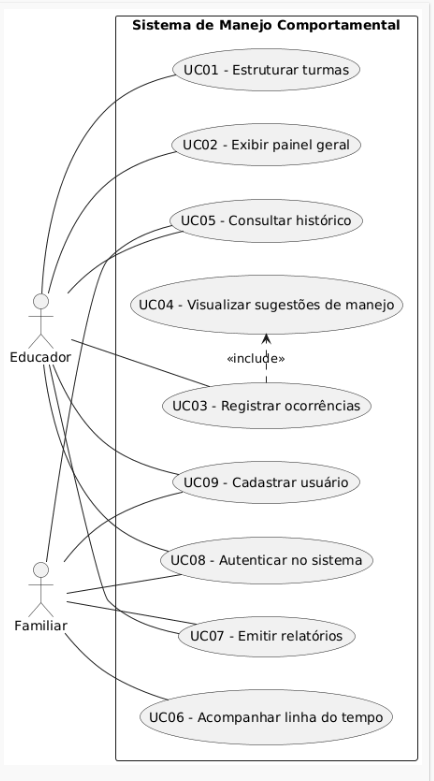
\includegraphics[width=0.3\textwidth, keepaspectratio]{dados/figuras/casoDeUso.png}
    
    \vspace{0.2cm}
    
    \begin{flushleft}
        \footnotesize Fonte: Elaborada pela autora (2026).
    \end{flushleft}
\end{figure}

Esses casos de uso reforçam o caráter pedagógico e de apoio clínico do sistema, oferecendo aos responsáveis um acompanhamento transparente e contínuo sobre a evolução comportamental do aluno. Dessa forma, a plataforma transcende a função de um simples diário escolar, atuando como uma ferramenta ativa que integra a família e a escola na aplicação de intervenções assertivas para o TDAH e o TOD.

\vspace{0.5cm}
\section{Protótipos}

Esta seção apresenta os protótipos de alta fidelidade desenvolvidos nas plataformas Figma \cite{figma2026} e Canva \cite{canva2026} para a aplicação web responsiva voltada ao suporte e manejo comportamental de alunos com TDAH e TOD. Os protótipos têm como objetivo representar o layout adaptável (para acesso em computadores institucionais e smartphones) e os principais elementos gráficos planejados para a implementação do sistema. A concepção das telas foi norteada por princípios de usabilidade e redução de carga cognitiva, adequando-se à realidade do público-alvo: professores com rotinas escolares aceleradas e familiares que buscam informações claras. Dessa forma, cada interface foi estruturada para oferecer uma navegação intuitiva, priorizando fluxos de registro ágeis, uma paleta de cores que transmite foco e acolhimento, e destaque visual imediato para as estratégias proativas de intervenção.

Para além do design, é fundamental compreender o fluxo operacional contínuo que rege a plataforma, estruturado para conectar as ações da escola ao acompanhamento da família. A jornada de uso inicia-se quando o educador acessa o sistema e visualiza o painel geral da sua turma, onde seleciona o perfil do aluno desejado. Diante de uma situação atípica, o professor registra a ocorrência de forma ágil. Imediatamente após o salvamento, o sistema processa o dado e exibe na tela cards com sugestões de manejo prático em tempo real. De forma simultânea, essa ação atualiza a linha do tempo (timeline) do estudante. Assim, a família pode acompanhar o histórico cronológico de eventos pelo celular, garantindo transparência e possibilitando a continuidade das abordagens terapêuticas no ambiente doméstico. A seguir, são detalhadas as telas que materializam esse fluxo.

\vspace{0.5cm}
\subsection{Tela de login}

A Figura 4.1 apresenta a tela inicial de autenticação (login) da plataforma. Nesta interface, o usuário é recebido por uma mensagem de boas-vindas e pelo lema "Educação com foco e cuidado". O destaque central da tela é a seleção do perfil de acesso, permitindo que o usuário identifique-se como “Educador” ou “Familiar” por meio de cartões amplos com ícones ilustrativos e intuitivos. Essa segregação inicial não é apenas visual, mas funcional: ela garante que o sistema direcione o educador para o painel de gestão da turma e o familiar para a linha do tempo do aluno, assegurando a privacidade dos dados de saúde e comportamento, conforme exigido pela LGPD.

Logo abaixo, encontram-se os campos minimalistas para a inserção das credenciais (e-mail e senha), atalhos para recuperação de acesso ou novo cadastro, e o botão principal ("Entrar"). O layout foi estruturado com base nos princípios de baixa carga cognitiva, utilizando cores suaves, amplo espaçamento em branco (white space) e áreas de toque facilitadas, garantindo uma navegação fluida tanto na versão desktop quanto na responsiva para dispositivos móveis.

\begin{figure}[H] 
    \centering
    \caption{Tela de login} % <-- Legenda ÚNICA no topo
    \label{fig:telas_login}
    \vspace{0.3cm}
    
    % --- Imagem A ---
    \begin{minipage}[b]{0.65\textwidth}
        \centering
        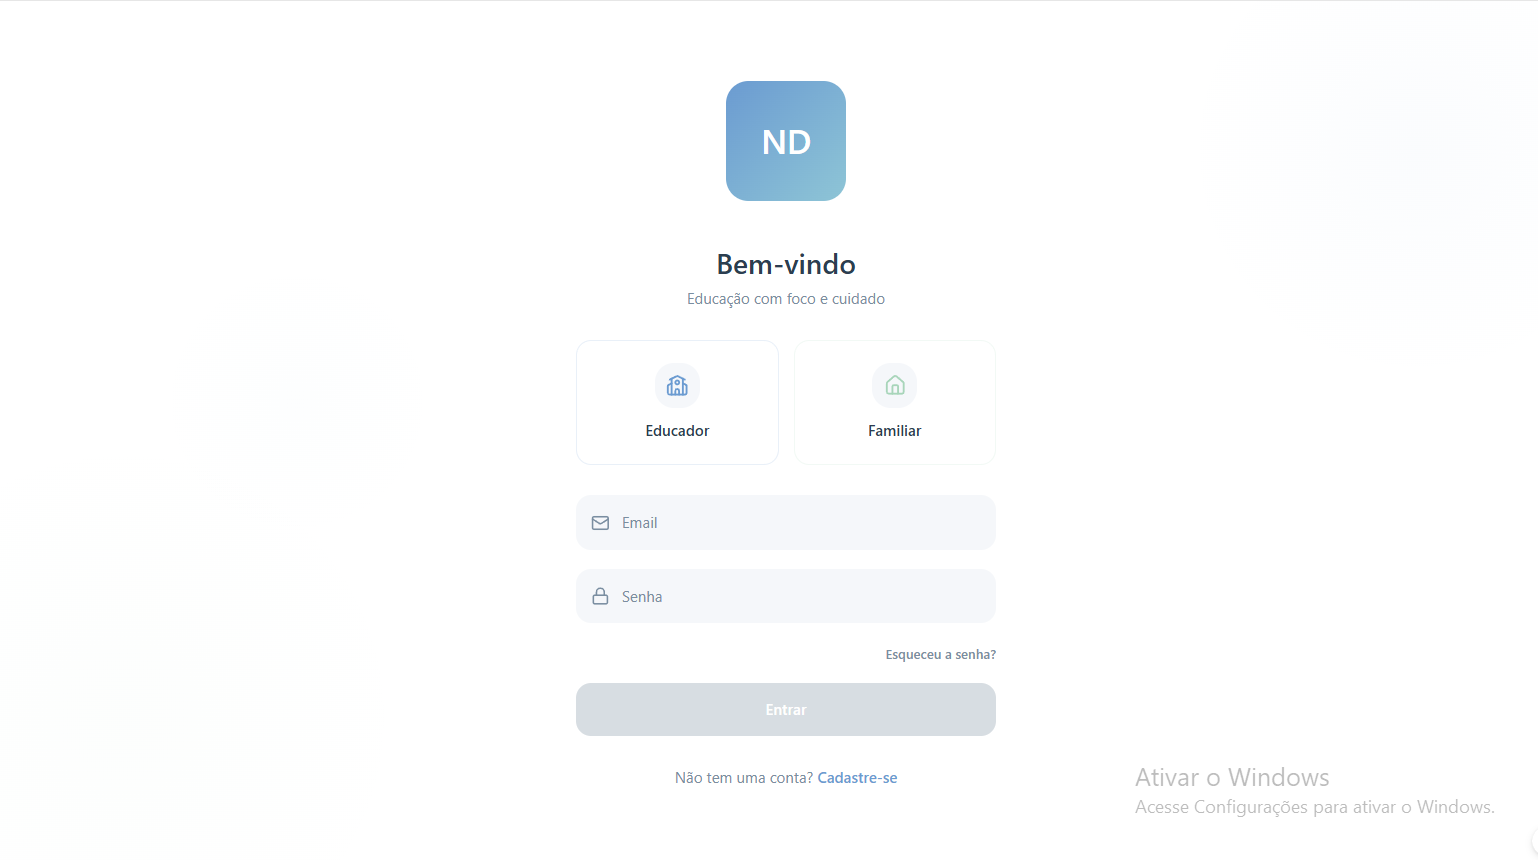
\includegraphics[height=9cm, keepaspectratio]{dados/figuras/telaLoginDesktop} 
        \centerline{\small (a) Desktop.} % <-- Subtítulo A
    \end{minipage}\hfill
    \rule{0.5pt}{10cm}\hfill % <-- 0.5pt é a espessura, 7cm é a altura
    % --- Imagem B ---
    \begin{minipage}[b]{0.30\textwidth}
        \centering
        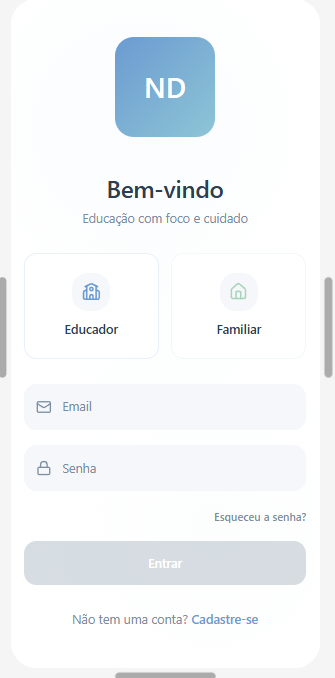
\includegraphics[height=9cm, keepaspectratio]{dados/figuras/telaLoginMobile}
        \centerline{\small (b) Mobile.} % <-- Subtítulo B
    \end{minipage}
    
   \vspace{0.3cm}
    \begin{flushleft} % <-- Inicia o alinhamento à esquerda
   \footnotesize{Fonte: Elaborada pela autora (2026).} % <-- Fonte ÚNICA no final
 \end{flushleft}   
\end{figure}

\vspace{0.5cm}
\subsection{Tela inicial para professor}

A Figura 4.2 apresenta o "Painel da Turma", a interface principal (dashboard) destinada ao perfil "Educador". O layout foi desenvolvido com foco primário na agilidade e na gestão visual, características essenciais para não sobrecarregar o docente durante a dinâmica da sala de aula. No topo da tela, destaca-se o botão de ação primária "+ Nova Ocorrência", dimensionado e posicionado estrategicamente para garantir o registro rápido de eventos comportamentais. 

    A listagem de alunos é apresentada por meio de cards minimalistas que incorporam indicadores visuais de status (pontos coloridos em tons suaves), permitindo ao professor monitorar o panorama da turma com uma leitura rápida e de baixo esforço cognitivo. Ademais, as telas evidenciam a arquitetura responsiva do sistema, demonstrando como a interface se adapta de forma fluida: operando em um formato de grade distribuída na visualização para computadores (desktop) e reorganizando-se automaticamente em uma lista vertical contínua na versão para dispositivos móveis (mobile), sem perda de funcionalidade ou usabilidade.

\begin{figure}[H] 
    \centering
    \caption{Tela inicial - professor} % <-- Legenda ÚNICA no topo
    \label{fig:telas_login}
    \vspace{0.3cm}
    
    % --- Imagem A ---
    \begin{minipage}[b]{0.65\textwidth}
        \centering
        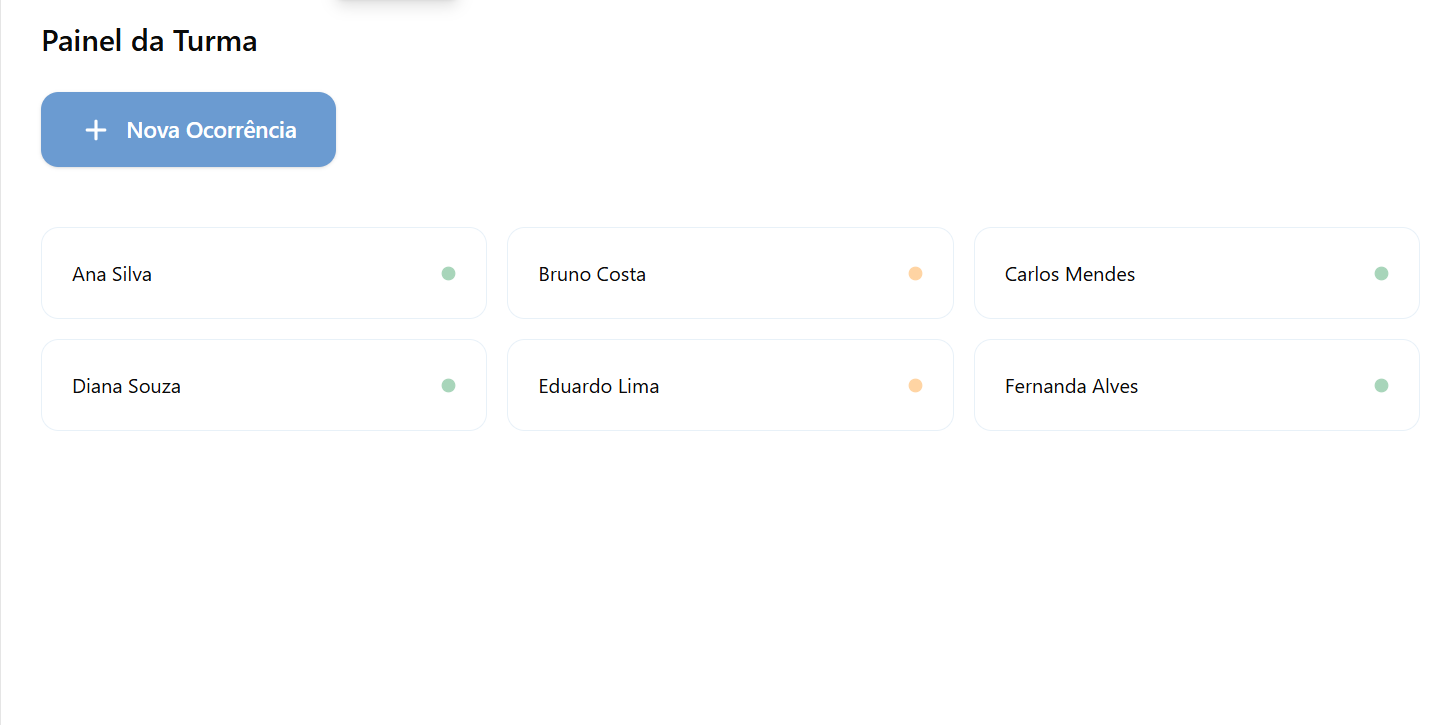
\includegraphics[height=9cm, keepaspectratio]{dados/figuras/telaInical_professorDesktop} 
        \centerline{\small (a) Desktop.} % <-- Subtítulo A
    \end{minipage}\hfill
    \rule{0.5pt}{10cm}\hfill % <-- 0.5pt é a espessura, 7cm é a altura
    % --- Imagem B ---
    \begin{minipage}[b]{0.30\textwidth}
        \centering
        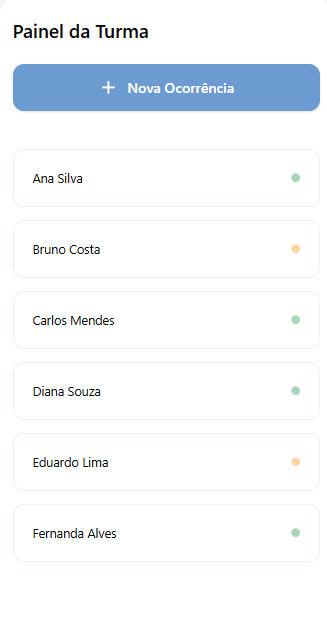
\includegraphics[height=9cm, keepaspectratio]{dados/figuras/telaInical_professorMobile}
        \centerline{\small (b) Mobile.} % <-- Subtítulo B
    \end{minipage}
    
   \vspace{0.3cm}
    \begin{flushleft} % <-- Inicia o alinhamento à esquerda
   \footnotesize{Fonte: Elaborada pela autora (2026).} % <-- Fonte ÚNICA no final
 \end{flushleft}   
\end{figure}

\vspace{0.5cm}
\subsection{Tela inicial para os familiares}

A Figura 4.3 ilustra a interface principal destinada ao perfil "Familiar", apresentada nas suas versões desktop e mobile. Em oposição a um painel de controlo complexo, esa tela adota o formato de uma linha do tempo (timeline) cronológica, assemelhando-se a um feed de atualizações. No topo, a identificação clara do aluno estabelece imediatamente o contexto de navegação. O corpo da interface exibe os registros diários — tais como comportamentos positivos, ocorrências de agitação e avisos pedagógicos — através de cards informativos, acompanhados da respetiva hora de registo. 

A utilização de ícones intuitivos e de uma paleta de cores funcional e suave (como o verde para atitudes colaborativas e o azul para alertas e ocorrências) permite uma compreensão visual imediata. A arquitetura responsiva garante que os familiares possam aceder à rotina escolar com clareza, tanto em computadores como em telefones, promovendo uma comunicação transparente e ágil entre a escola e a família, sempre a respeitar o princípio de baixa carga cognitiva.

\begin{figure}[H] 
    \centering
    \caption{Tela inicial - familiares} % <-- Legenda ÚNICA no topo
    \label{fig:telas_login}
    \vspace{0.3cm}
    
    % --- Imagem A ---
    \begin{minipage}[b]{0.65\textwidth}
        \centering
        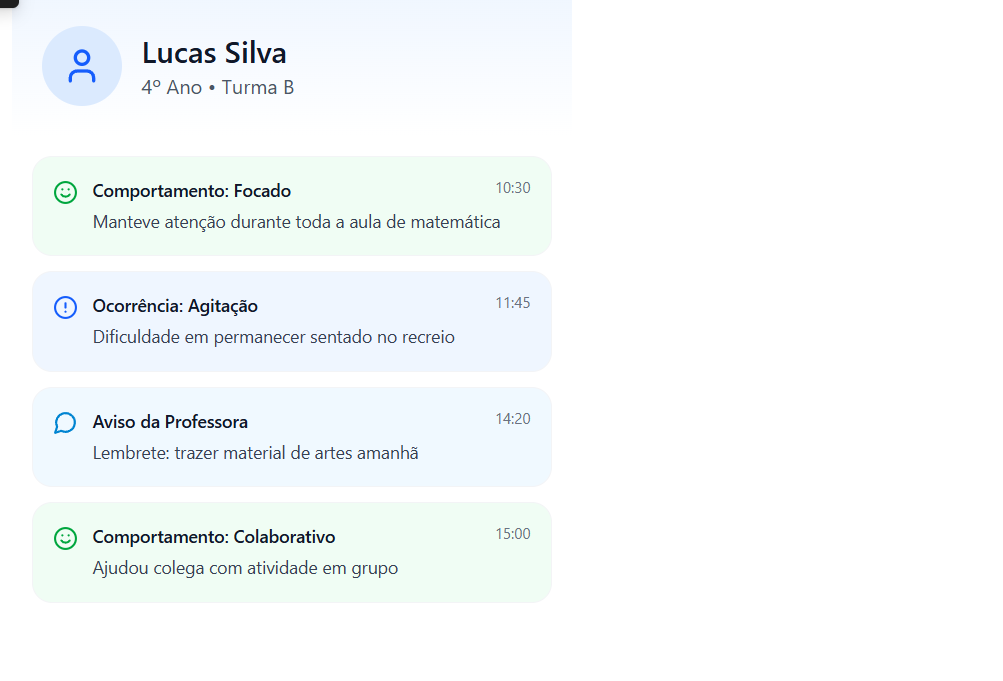
\includegraphics[height=9cm, keepaspectratio]{dados/figuras/telaInical_familiarDesktop} 
        \centerline{\small (a) Desktop.} % <-- Subtítulo A
    \end{minipage}\hfill
    \rule{0.5pt}{10cm}\hfill % <-- 0.5pt é a espessura, 7cm é a altura
    % --- Imagem B ---
    \begin{minipage}[b]{0.30\textwidth}
        \centering
        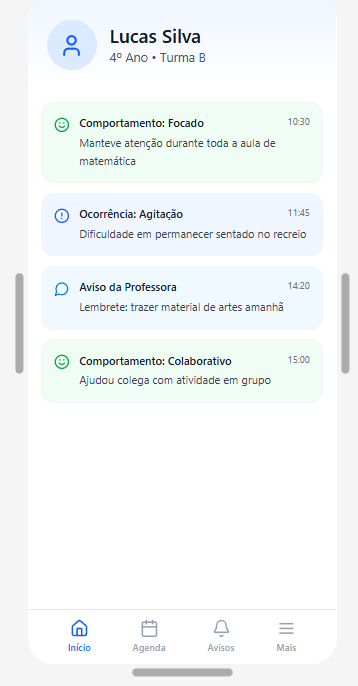
\includegraphics[height=9cm, keepaspectratio]{dados/figuras/telaInical_familiarMobile}
        \centerline{\small (b) Mobile.} % <-- Subtítulo B
    \end{minipage}
    
   \vspace{0.3cm}
    \begin{flushleft} % <-- Inicia o alinhamento à esquerda
   \footnotesize{Fonte: Elaborada pela autora (2026).} % <-- Fonte ÚNICA no final
 \end{flushleft}   
\end{figure}

\vspace{0.5cm}
\subsection{Tela de registro de ocorrências}

A Figura 4.4 ilustra o ecrã de novo registo de ocorrências, desenvolvido em exclusivo para o perfil de educador, apresentado nas suas vertentes mobile e desktop. O design desta interface foi concebido com foco absoluto na agilidade e na otimização do tempo, uma exigência crítica para não interromper a dinâmica da sala de aula. Para tal, minimizou-se a dependência de campos de texto livre, substituindo-os por botões de seleção rápida (chips ou tags) que categorizam os comportamentos típicos do TDAH e TOD (como agitação, desatenção e impulsividade) e os seus respectivos níveis de intensidade. 

O campo para observações textuais foi mantido estritamente como opcional. Esta abordagem não só padroniza a recolha de dados, como também reduz drasticamente a carga cognitiva exigida ao professor no momento de uma crise. Por fim, o botão de ação primária ("Salvar e Ver Sugestões") evidencia o grande diferencial do sistema: a transição imediata do registo passivo para o suporte pedagógico proativo.

\begin{figure}[H] 
    \centering
    \caption{Tela de registro de ocorrências} % <-- Legenda ÚNICA no topo
    \label{fig:telas_login}
    \vspace{0.3cm}
    
    % --- Imagem A ---
    \begin{minipage}[b]{0.65\textwidth}
        \centering
        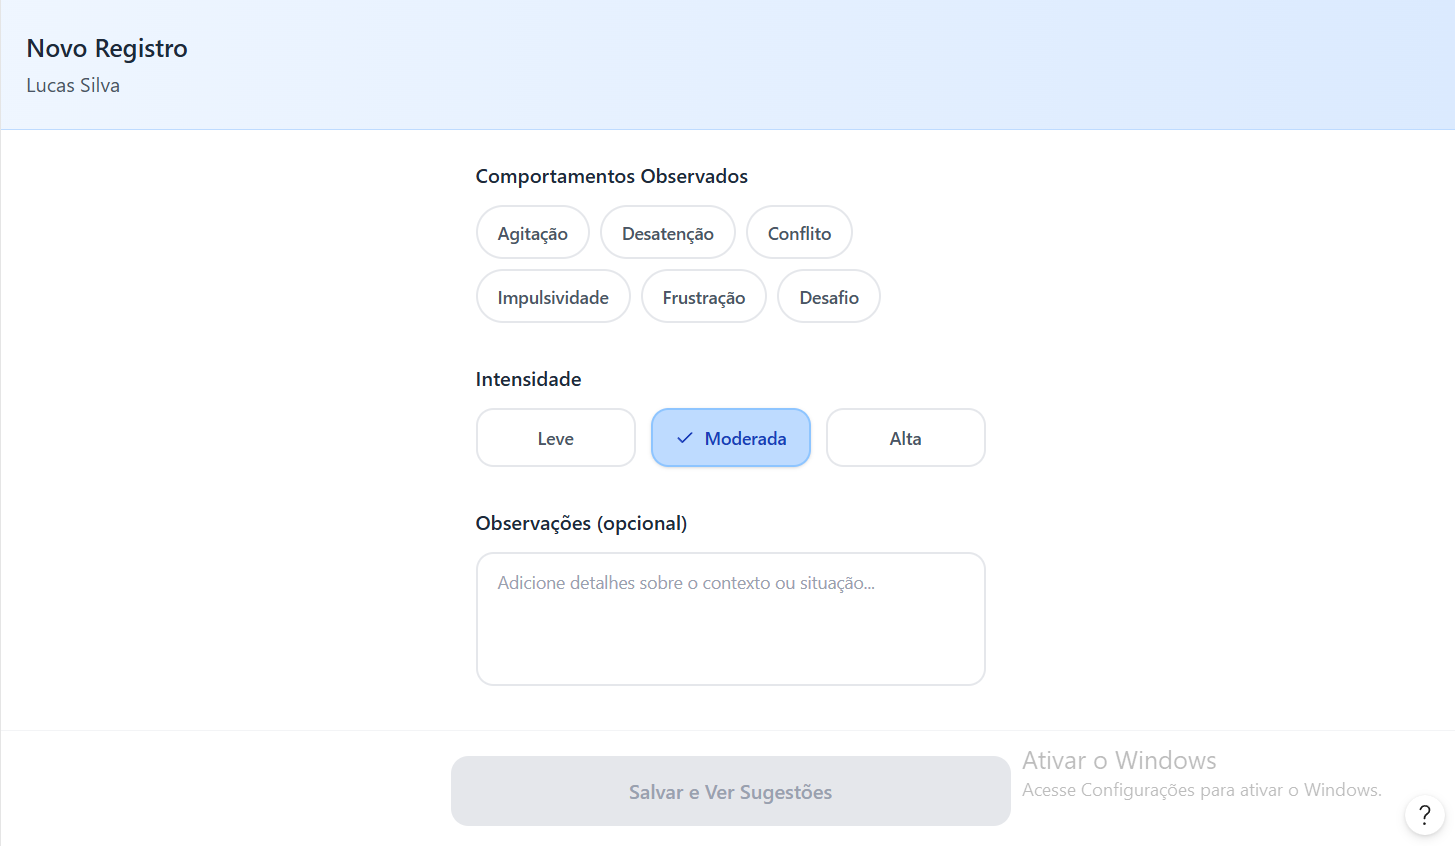
\includegraphics[height=9cm, keepaspectratio]{dados/figuras/ocorrenciasDesktop} 
        \centerline{\small (a) Desktop.} % <-- Subtítulo A
    \end{minipage}\hfill
    \rule{0.5pt}{10cm}\hfill % <-- 0.5pt é a espessura, 7cm é a altura
    % --- Imagem B ---
    \begin{minipage}[b]{0.30\textwidth}
        \centering
        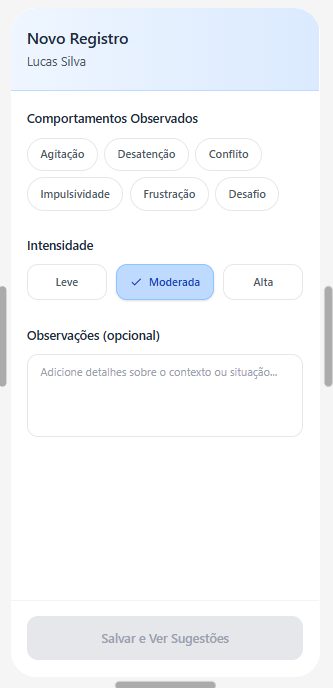
\includegraphics[height=9cm, keepaspectratio]{dados/figuras/ocorrenciasMobile}
        \centerline{\small (b) Mobile.} % <-- Subtítulo B
    \end{minipage}
    
   \vspace{0.3cm}
    \begin{flushleft} % <-- Inicia o alinhamento à esquerda
   \footnotesize{Fonte: Elaborada pela autora (2026).} % <-- Fonte ÚNICA no final
 \end{flushleft}   
\end{figure}

\vspace{0.5cm}
\subsection{Tela de estratégias de manejo}

A Figura 4.5 apresenta a interface de Estratégias de Manejo, que constitui o principal diferencial pedagógico e tecnológico da plataforma. Ao concluir o registro de uma ocorrência, o educador é imediatamente direcionado para esta tela, que atua como um assistente proativo. Em vez de apenas armazenar passivamente o dado comportamental, o sistema filtra e exibe cards com sugestões de intervenção baseadas em evidências para o TDAH e TOD, contextualizadas com o comportamento recém-registrado (como, por exemplo, pausas para movimento ou reforço positivo imediato). 

O design da interface mantém a coerência visual das telas anteriores, priorizando o baixo peso cognitivo: as instruções são curtas, objetivas e acompanhadas de ícones claros, garantindo que o professor possa ler e aplicar a estratégia em questão de segundos, promovendo a autorregulação do aluno e a minimização de conflitos no ambiente escolar.

\begin{figure}[H] 
    \centering
    \caption{Tela de registro de ocorrências} % <-- Legenda ÚNICA no topo
    \label{fig:telas_login}
    \vspace{0.3cm}
    
    % --- Imagem A ---
    \begin{minipage}[b]{0.65\textwidth}
        \centering
        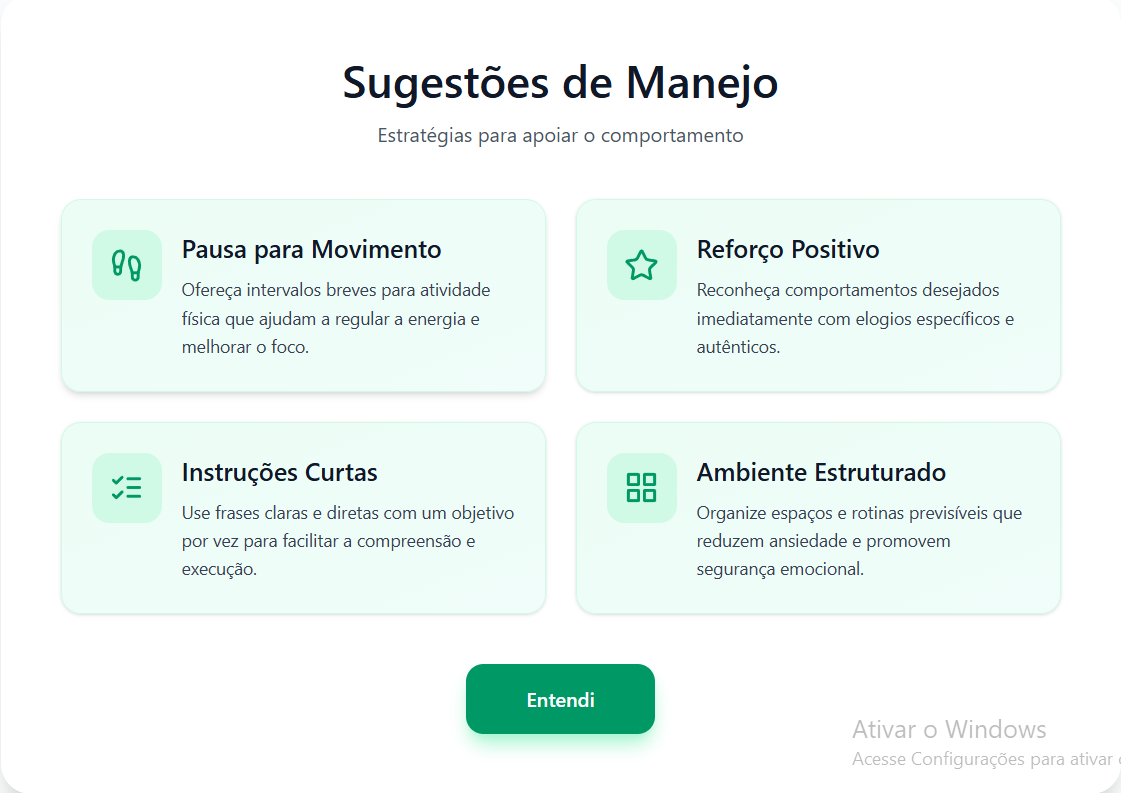
\includegraphics[height=9cm, keepaspectratio]{dados/figuras/estrategiaDeManejo_desktop} 
        \centerline{\small (a) Desktop.} % <-- Subtítulo A
    \end{minipage}\hfill
    \rule{0.5pt}{10cm}\hfill % <-- 0.5pt é a espessura, 7cm é a altura
    % --- Imagem B ---
    \begin{minipage}[b]{0.30\textwidth}
        \centering
        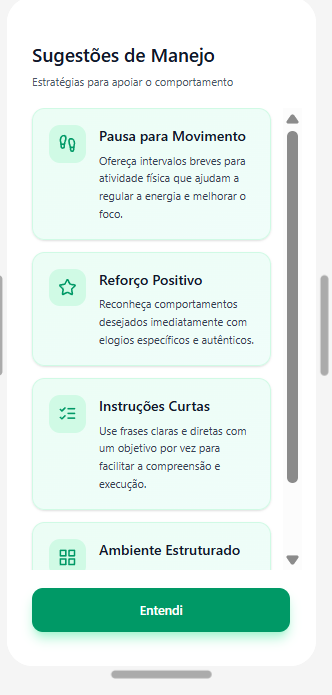
\includegraphics[height=9cm, keepaspectratio]{dados/figuras/estrategiaDeManejo_mobile}
        \centerline{\small (b) Mobile.} % <-- Subtítulo B
    \end{minipage}
    
   \vspace{0.3cm}
    \begin{flushleft} % <-- Inicia o alinhamento à esquerda
   \footnotesize{Fonte: Elaborada pela autora (2026).} % <-- Fonte ÚNICA no final
 \end{flushleft}   
\end{figure}

\vspace{0.5cm}
\subsection{Tela da linha do tempo da família}

A Figura 4.6 apresenta a tela de histórico diário do aluno, estruturada em formato de linha do tempo (timeline), em suas versões mobile e desktop. Esta interface funciona como o principal canal de acompanhamento para a família e como registro de consulta para o educador. O layout reforça a premissa de baixa carga cognitiva ao destacar, no topo, a identificação clara do estudante. O fluxo central é composto por cards de eventos organizados cronologicamente, que empregam uma categorização visual baseada em cores e ícones específicos: verde para comportamentos positivos e foco, azul para avisos ou comunicações neutras, e laranja para alertas comportamentais de agitação. 

Essa sinalização visual permite aos usuários uma assimilação imediata do estado do aluno, sem a necessidade de uma leitura exaustiva. Adicionalmente, as imagens evidenciam a arquitetura responsiva do sistema, ilustrando a adaptação da barra de navegação — posicionada no rodapé nos celulares e na lateral esquerda nos computadores — de modo a preservar a ergonomia e a acessibilidade em qualquer dispositivo.

\begin{figure}[H] 
    \centering
    \caption{Tela da linha do tempo da família} % <-- Legenda ÚNICA no topo
    \label{fig:telas_login}
    \vspace{0.3cm}
    
    % --- Imagem A ---
    \begin{minipage}[b]{0.65\textwidth}
        \centering
        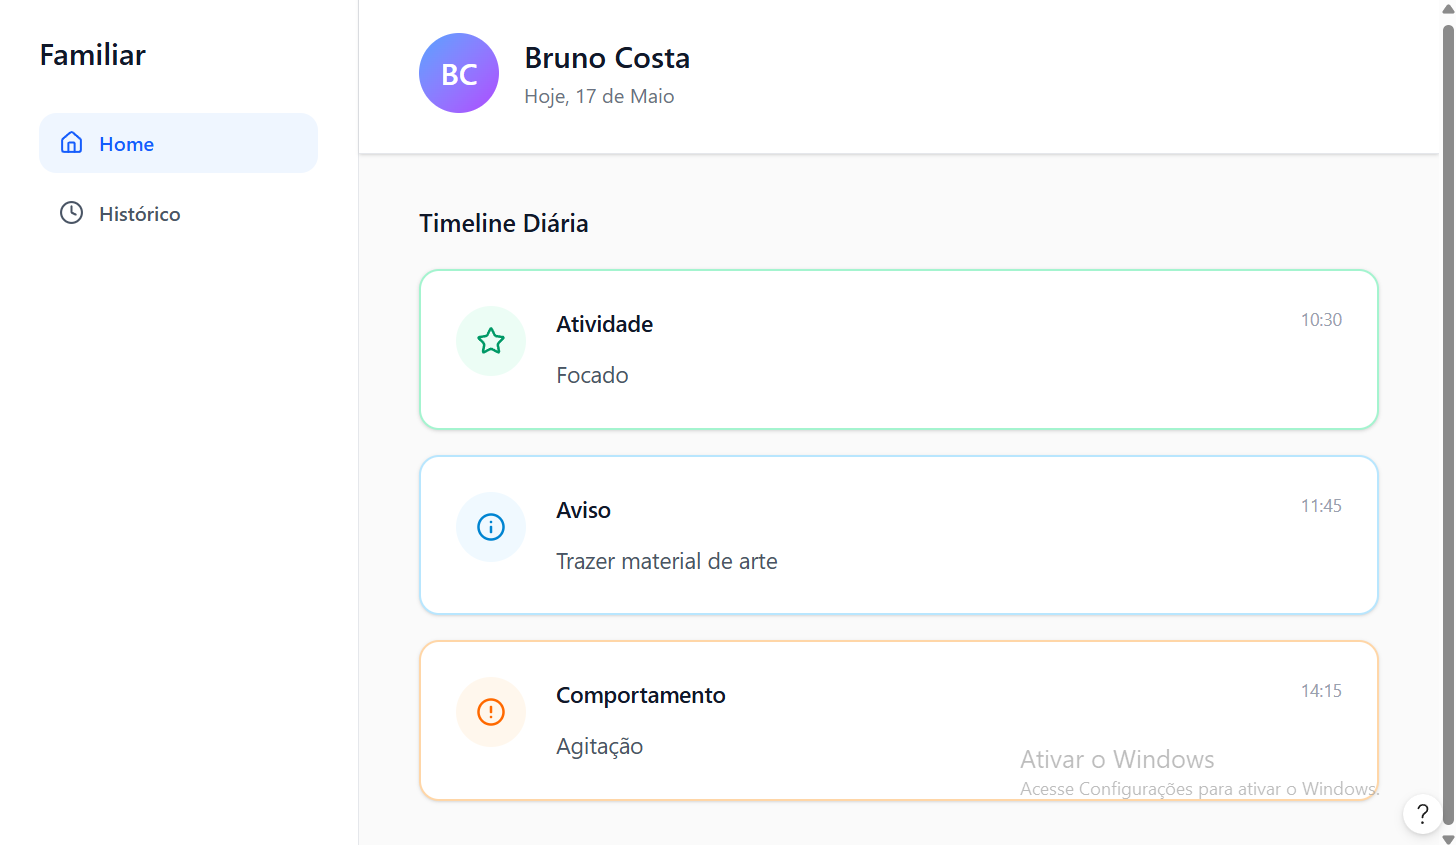
\includegraphics[height=9cm, keepaspectratio]{dados/figuras/timeline_Desktop} 
        \centerline{\small (a) Desktop.} % <-- Subtítulo A
    \end{minipage}\hfill
    \rule{0.5pt}{10cm}\hfill % <-- 0.5pt é a espessura, 7cm é a altura
    % --- Imagem B ---
    \begin{minipage}[b]{0.30\textwidth}
        \centering
        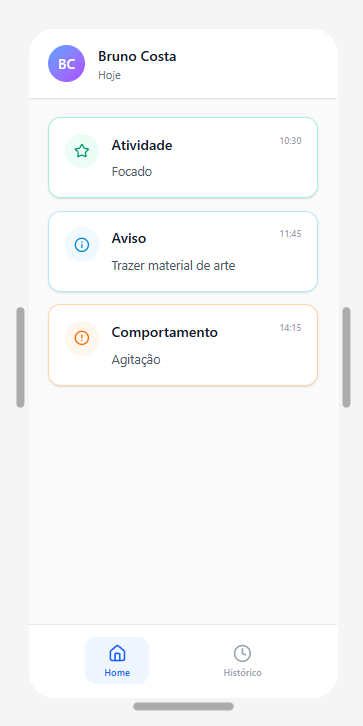
\includegraphics[height=9cm, keepaspectratio]{dados/figuras/timelineMobile}
        \centerline{\small (b) Mobile.} % <-- Subtítulo B
    \end{minipage}
    
   \vspace{0.3cm}
    \begin{flushleft} % <-- Inicia o alinhamento à esquerda
   \footnotesize{Fonte: Elaborada pela autora (2026).} % <-- Fonte ÚNICA no final
 \end{flushleft}   
\end{figure}       
    % ----------------------------------------------------------------------------
%                               Conclusão
% ----------------------------------------------------------------------------
\chapter{Conclusão}
\label{chap:conclusão}

O presente trabalho teve como objetivo central investigar e propor uma solução tecnológica voltada ao suporte pedagógico e ao manejo comportamental de alunos com Transtorno do Déficit de Atenção com Hiperatividade (TDAH) e Transtorno Opositivo Desafiador (TOD). Por meio do levantamento de requisitos e da subsequente prototipagem de alta fidelidade, foi possível materializar uma aplicação web responsiva que visa atender às demandas latentes da comunidade escolar.

A principal contribuição deste projeto reside na proposição de uma transição do modelo de registro passivo para uma abordagem de manejo proativo. A interface desenvolvida, estruturada sob os princípios de usabilidade e baixa carga cognitiva, apresenta-se como uma alternativa viável para o dinâmico contexto escolar. A substituição de formulários extensos por seleções ágeis (chips) e a entrega imediata de estratégias de intervenção baseadas em evidências têm o potencial de reduzir significativamente a sobrecarga do corpo docente em momentos de crise.

Paralelamente, a estruturação de uma linha do tempo (timeline) dedicada aos familiares democratiza o acesso à informação, promovendo uma comunicação transparente e livre de ruídos entre a escola e o ambiente doméstico. Essa arquitetura reafirma a importância da tecnologia não apenas como ferramenta de arquivamento, mas como ponte para a construção de uma rede de apoio colaborativa em prol do desenvolvimento do estudante neurodivergente.

Devido às restrições temporais inerentes ao escopo deste trabalho, a etapa de validação prática da ferramenta em ambiente escolar e a aplicação de testes de usabilidade com o público-alvo não puderam ser realizadas. Como trabalhos futuros, sugere-se a implementação do código-fonte da aplicação web com base nos requisitos levantados, seguida de um estudo de caso prático no Instituto Federal de Brasília (IFB), visando avaliar o impacto real e a aplicabilidade dos cards de manejo proativo na rotina dos educadores e das famílias.                 			     % Conclusão
    
    \postextual
    % Insere elementos pós-textuais
    \include{estrutura/pos-textuais/referencias}           			   % Referências
    \addcontentsline{toc}{chapter}{APÊNDICES} % Adiciona a palavra APÊNDICES ao Sumário
\begin{apendicesenv}

\chapter{Questionário de Levantamento de Requisitos e Necessidades com Educadores}
\label{ap:questionario_educadores}

Este apêndice apresenta o instrumento de pesquisa (questionário) estruturado e direcionado a professores e profissionais da educação, com o objetivo de coletar informações sobre as principais dores, desafios na rotina escolar e requisitos funcionais para o suporte ao manejo comportamental de alunos com TDAH e TOD.

\begin{enumerate}
    \item \textbf{Qual é o seu tempo de atuação na área da educação?}
    \begin{itemize}
        \item[ ] Menos de 2 anos
        \item[ ] De 2 a 5 anos
        \item[ ] De 5 a 10 anos
        \item[ ] Mais de 10 anos
    \end{itemize}
    
    \item \textbf{Com que frequência você atua ou já atuou com alunos diagnosticados com TDAH ou TOD em sala de aula?}
    \begin{itemize}
        \item[ ] Frequentemente (rotina diária)
        \item[ ] Ocasionalmente
        \item[ ] Raramente
        \item[ ] Nunca atuei
    \end{itemize}

    \item \textbf{Quais são os maiores desafios encontrados no momento de documentar e registrar crises ou comportamentos atípicos desses alunos? (Selecione mais de uma opção, se aplicável)}
    \begin{itemize}
        \item[ ] Falta de tempo hábil durante o período de aula.
        \item[ ] Formulários institucionais extensos ou complexos.
        \item[ ] Falta de um canal direto e rápido para reportar à coordenação/família.
        \item[ ] Dificuldade em lembrar dos detalhes do ocorrido após o término do turno.
    \end{itemize}

    \item \textbf{No momento em que ocorre uma crise comportamental em sala de aula, você sente que possui fácil acesso a estratégias de manejo imediato baseadas em evidências?}
    \begin{itemize}
        \item[ ] Sim, sempre sei como intervir de forma padronizada.
        \item[ ] Parcialmente, mas sinto falta de suporte proativo ou sugestões rápidas.
        \item[ ] Não, geralmente preciso recorrer à coordenação ou agir por intuição no momento.
    \end{itemize}

    \item \textbf{Como é realizada, atualmente, a comunicação com os familiares para relatar o comportamento e a evolução diária do aluno?}
    \begin{itemize}
        \item[ ] Agenda física escolar escolar.
        \item[ ] Aplicativos de mensagem (como WhatsApp).
        \item[ ] Reuniões periódicas presenciais.
        \item[ ] Não há um fluxo constante de comunicação diária.
    \end{itemize}

    \item \textbf{Em sua visão, o quão útil seria uma aplicação web responsiva (acessível por computador ou celular) que permitisse registrar ocorrências de forma ágil (usando \textit{chips}/seleções rápidas) e que entregasse imediatamente sugestões práticas de manejo pedagógico?}
    \begin{itemize}
        \item[ ] Extremamente útil (otimizaria a rotina).
        \item[ ] Muito útil.
        \item[ ] Indiferente.
        \item[ ] Pouco útil.
    \end{itemize}
\end{enumerate}

\end{apendicesenv}

\end{document}
